% ATTENZIONE: Nei file secondari NON devi inserire \begin{document} o \end{document}.
\newpage

\chapterimage{Pictures/Indice.png}
\chapter{Sequence Models}\label{ch:sequence_models}

\section{Introduction to Sequence Modeling}

Standard feedforward architectures (such as multi-layer perceptrons and traditional convolutional neural networks) operate strictly under a \textbf{one-to-one} paradigm: a fixed-dimensional input vector $x \in \mathbb{R}^D$ is mapped to a fixed-dimensional output $y \in \mathbb{R}^K$. While effective for static tasks like single-image classification, this formulation fails when dealing with data that unfolds over time or possesses an intrinsic sequential nature, such as text, audio, video streams, or financial time series. This chapter covers sequence modeling paradigms, recurrent neural networks, and gating mechanisms based on the course lecture slides~\cite{galasso2025seqmodels}.

\begin{keywordbox}
\textbf{The Sequence Modeling Challenge} \\
In sequential tasks, either the input, the output, or both can have arbitrary and variable lengths:
\[ \{x_1, x_2, \dots, x_T\} \quad \longrightarrow \quad \{y_1, y_2, \dots, y_{T'}\} \]
A sequence model must be able to preserve temporal order, handle variable-length sequences without retraining, and share learned parameters across different time steps.
\end{keywordbox}

\subsection{Taxonomy of Sequence Tasks}

Depending on whether the input and output consist of single vectors or sequences of vectors, sequential problems are traditionally classified into five primary architectural paradigms, illustrated in Figure~\ref{fig:seq_taxonomy}.

\begin{figure}[htbp]
    \centering
    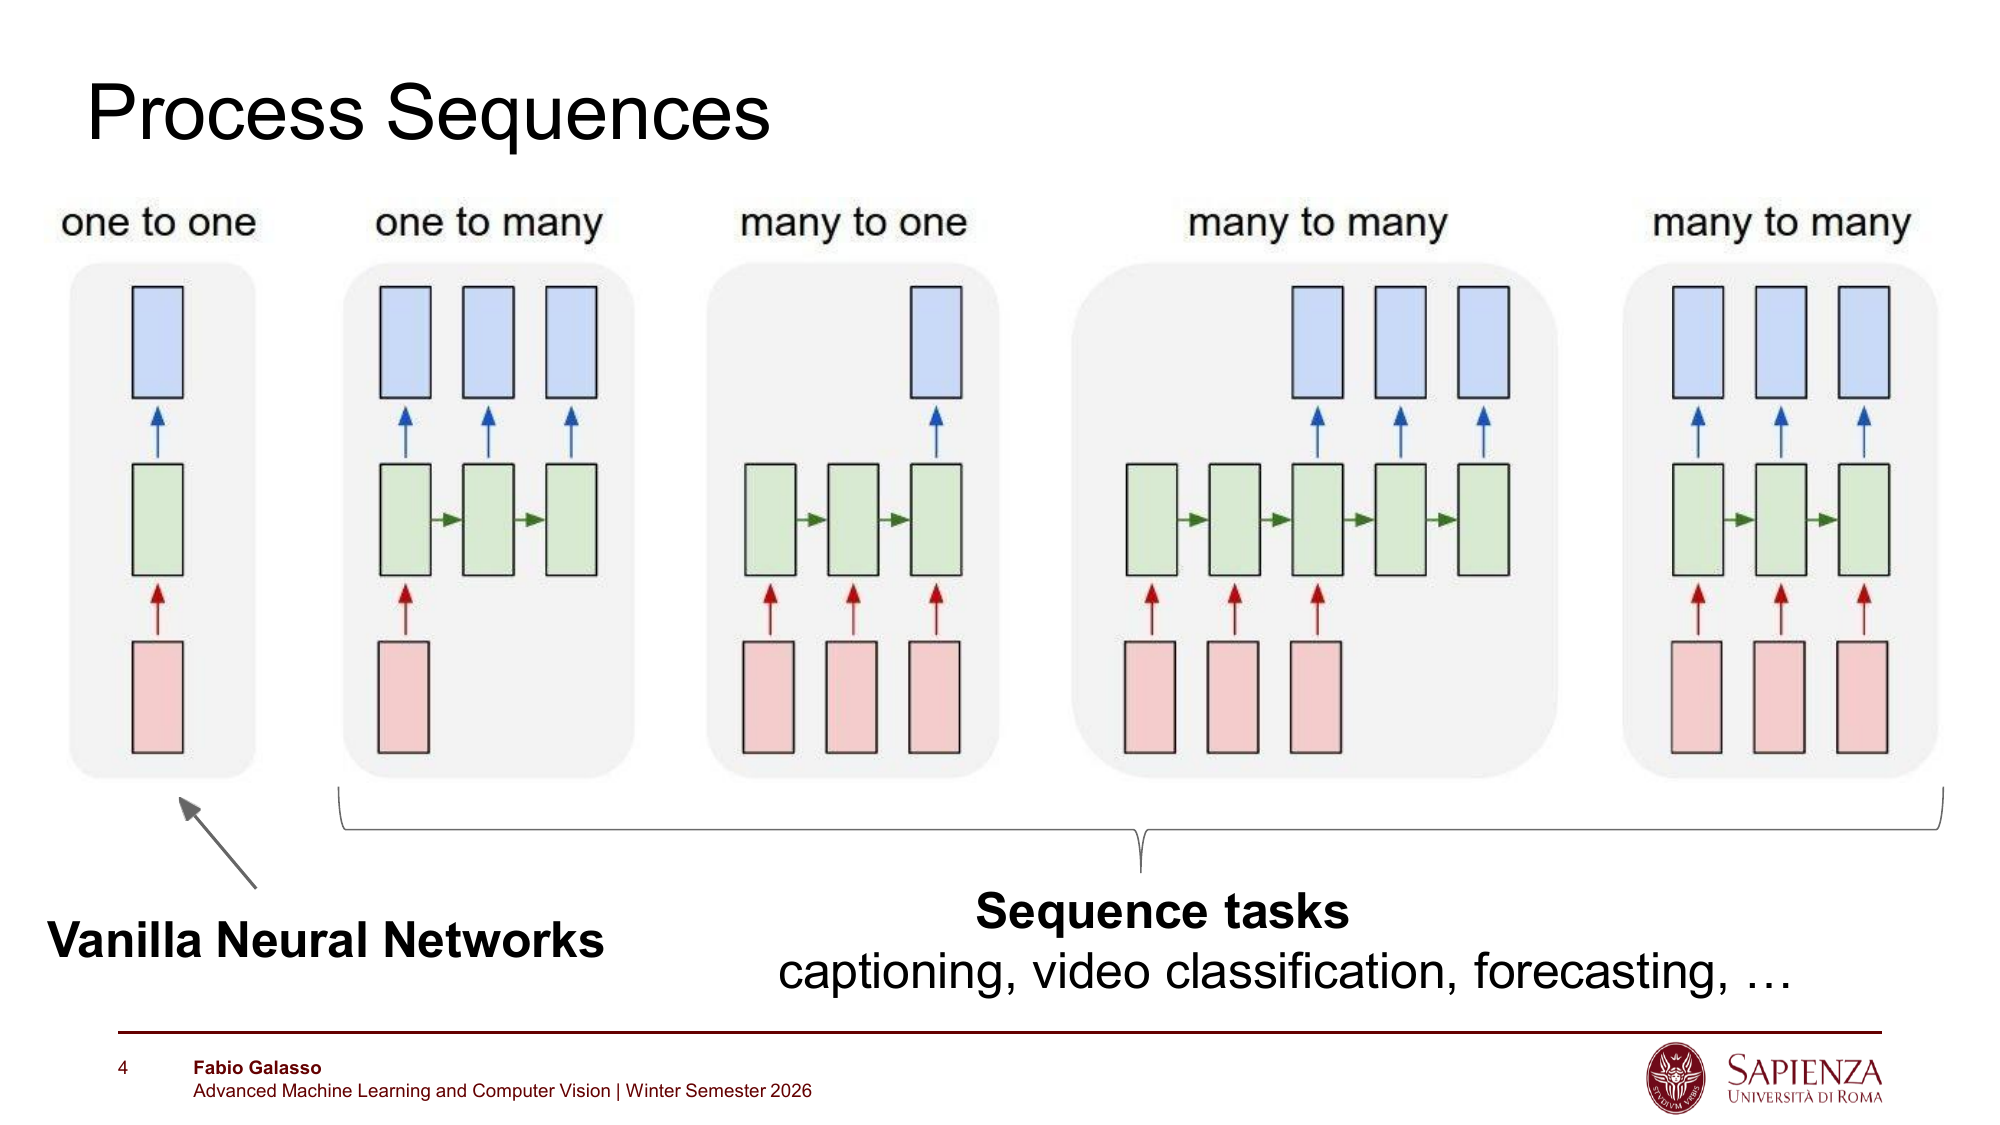
\includegraphics[width=0.85\textwidth]{Pictures/seq_taxonomy.png}
    \caption{Architectural taxonomy of sequence processing tasks (from course slides). Pink boxes denote inputs, green boxes represent internal processing units, and blue boxes denote outputs.}\label{fig:seq_taxonomy}
\end{figure}

\begin{itemize}[leftmargin=*]
    \item \textbf{One-to-One:} The conventional neural network setup without temporal recurrence. A single input produces a single output (e.g., standard image classification).
    \item \textbf{One-to-Many:} A single fixed-size input generates a sequential output of variable length. A prominent example is \textbf{Image Captioning}, where a single visual input (e.g., a photo of a dog) produces an output sequence of textual tokens (\textit{``A happy brown dog''}).
    \item \textbf{Many-to-One:} A temporal sequence of inputs is processed and summarized into a single static prediction. Typical examples include \textbf{Action Prediction / Video Classification} (where a temporal sequence of consecutive video frames is mapped to a single discrete action label like \textit{``Jumping''}) and \textbf{Sentiment Analysis} (a sequence of words mapped to a positive or negative score).
    \item \textbf{Many-to-Many (Synchronized / Aligned):} Both input and output are sequences of equal length, evaluated in lockstep at every time step. An example is \textbf{Frame-level Video Classification}, where an action category or segmentation map is predicted synchronously for each incoming frame.
    \item \textbf{Many-to-Many (Asynchronous / Sequence-to-Sequence):} The input sequence and output sequence have independent lengths ($T \neq T'$). This paradigm powers \textbf{Machine Translation} (translating an English sentence into Italian) and \textbf{Video Captioning} (ingesting a sequence of video frames to output a descriptive sentence, e.g., \textit{``A dog jumps over a hurdle''}).
\end{itemize}

\subsection{Forecasting as a Core Sequence Problem}

A critical subset of sequence tasks is \textbf{Forecasting}: given a historical trajectory or sequence of observations up to the current time $t$, predict future observations:
\[ (x_1, x_2, \dots, x_t) \quad \longrightarrow \quad (\hat{x}_{t+1}, \hat{x}_{t+2}, \dots) \]

\begin{examplebox}
\textbf{Real-World Applications of Forecasting:}
\begin{itemize}[nosep, leftmargin=*]
    \item \textbf{Trajectory Forecasting:} Predicting the future spatial paths of pedestrians and vehicles, essential for collision avoidance in autonomous driving and human-robot interaction.
    \item \textbf{Long-term Tracking across Occlusions:} Estimating the motion of targets when temporarily blocked by obstacles.
    \item \textbf{Physical and Financial Time Series:} Forecasting weather patterns, seismic alerts, critical pressure thresholds in industrial power plants, and financial market trends.
\end{itemize}
\end{examplebox}

---

\section{Temporal Convolutional Networks}

Before exploring recurrent architectures, sequence modeling can be approached using \textbf{Convolutional Neural Networks} applied along the temporal dimension, commonly known as \textbf{Temporal Convolutional Networks (TCN)}.

\subsection{One-Dimensional Convolutions on Sequences}

While standard computer vision uses 2D convolutions over spatial grids, temporal data is structured as a 1D sequence over discrete time. The 1D discrete convolution of an input sequence $f$ with a learnable filter $g$ is formulated as:

\begin{equation}
(f * g)(i) = \sum_{k} g(k) \, f(i - k)
\label{eq:1d_conv}
\end{equation}

\begin{Notebox}
\textbf{Piece-by-Piece Mathematical Breakdown of Equation~\ref{eq:1d_conv}:}
\begin{itemize}[nosep, leftmargin=*]
    \item $i$: The discrete temporal index (time step) at which the output feature is evaluated.
    \item $f$: The 1D input sequence signal across time (e.g., raw temporal measurements or feature embeddings).
    \item $g$: The learnable convolutional kernel (filter) of fixed size $K$.
    \item $k$: The kernel offset index running over the temporal window of the filter ($k \in \{0, \dots, K-1\}$).
    \item $g(k)$: The learnable parameter (weight) at relative offset $k$ within the kernel.
    \item $f(i - k)$: The input value sampled $k$ time steps prior to time step $i$.
    \item $\sum_k$: The summation accumulating the weighted products across the entire receptive span of the kernel.
\end{itemize}
\end{Notebox}

\subsection{Causal and Dilated Convolutions}

When applying convolutions to sequential forecasting, two structural constraints arise:

\subsubsection{Causal Convolutions}
Standard convolutions compute outputs using a symmetric window that looks both backward and forward in time. For temporal prediction, accessing future time steps ($i+k$ with $k > 0$) causes an illegal information leak (\textit{lookahead}). Therefore, the convolution must be strictly \textbf{causal}: the calculation at time step $t$ depends solely on inputs $x_s$ where $s \le t$.

\subsubsection{Dilated Convolutions and Receptive Field}
A fundamental limitation of standard causal convolutions is that the \textbf{receptive field} (the maximum historical context the network can observe) grows only \textit{linearly} with the depth of the network:
\[ \text{Receptive Field} = 1 + L(K - 1) \]
where $L$ is the number of layers and $K$ is the kernel size. Capturing long-term temporal dependencies would therefore require an impractical number of layers.

To overcome this limitation, TCNs introduce \textbf{Dilated Causal Convolutions}, as illustrated in Figure~\ref{fig:tcn_dilated}. For a 1D sequence $f$ and kernel $g$, a dilated convolution with dilation factor $d$ is defined as:

\begin{equation}
(f *_d g)(i) = \sum_{k} g(k) \, f(i - d \cdot k)
\label{eq:dilated_conv}
\end{equation}

\begin{Notebox}
\textbf{Piece-by-Piece Mathematical Breakdown of Equation~\ref{eq:dilated_conv}:}
\begin{itemize}[nosep, leftmargin=*]
    \item $d$: The \textbf{dilation factor}, which determines the spacing between kernel taps. For $d=1$, Equation~\ref{eq:dilated_conv} reduces to a standard convolution. For $d > 1$, the filter samples inputs every $d$ steps, skipping $d-1$ intermediate values.
    \item $i - d \cdot k$: The temporal sampling index, stretching the effective reach of the kernel backwards in time without adding extra parameters.
\end{itemize}
\end{Notebox}

\newpage

\begin{figure}[htbp]
    \centering
    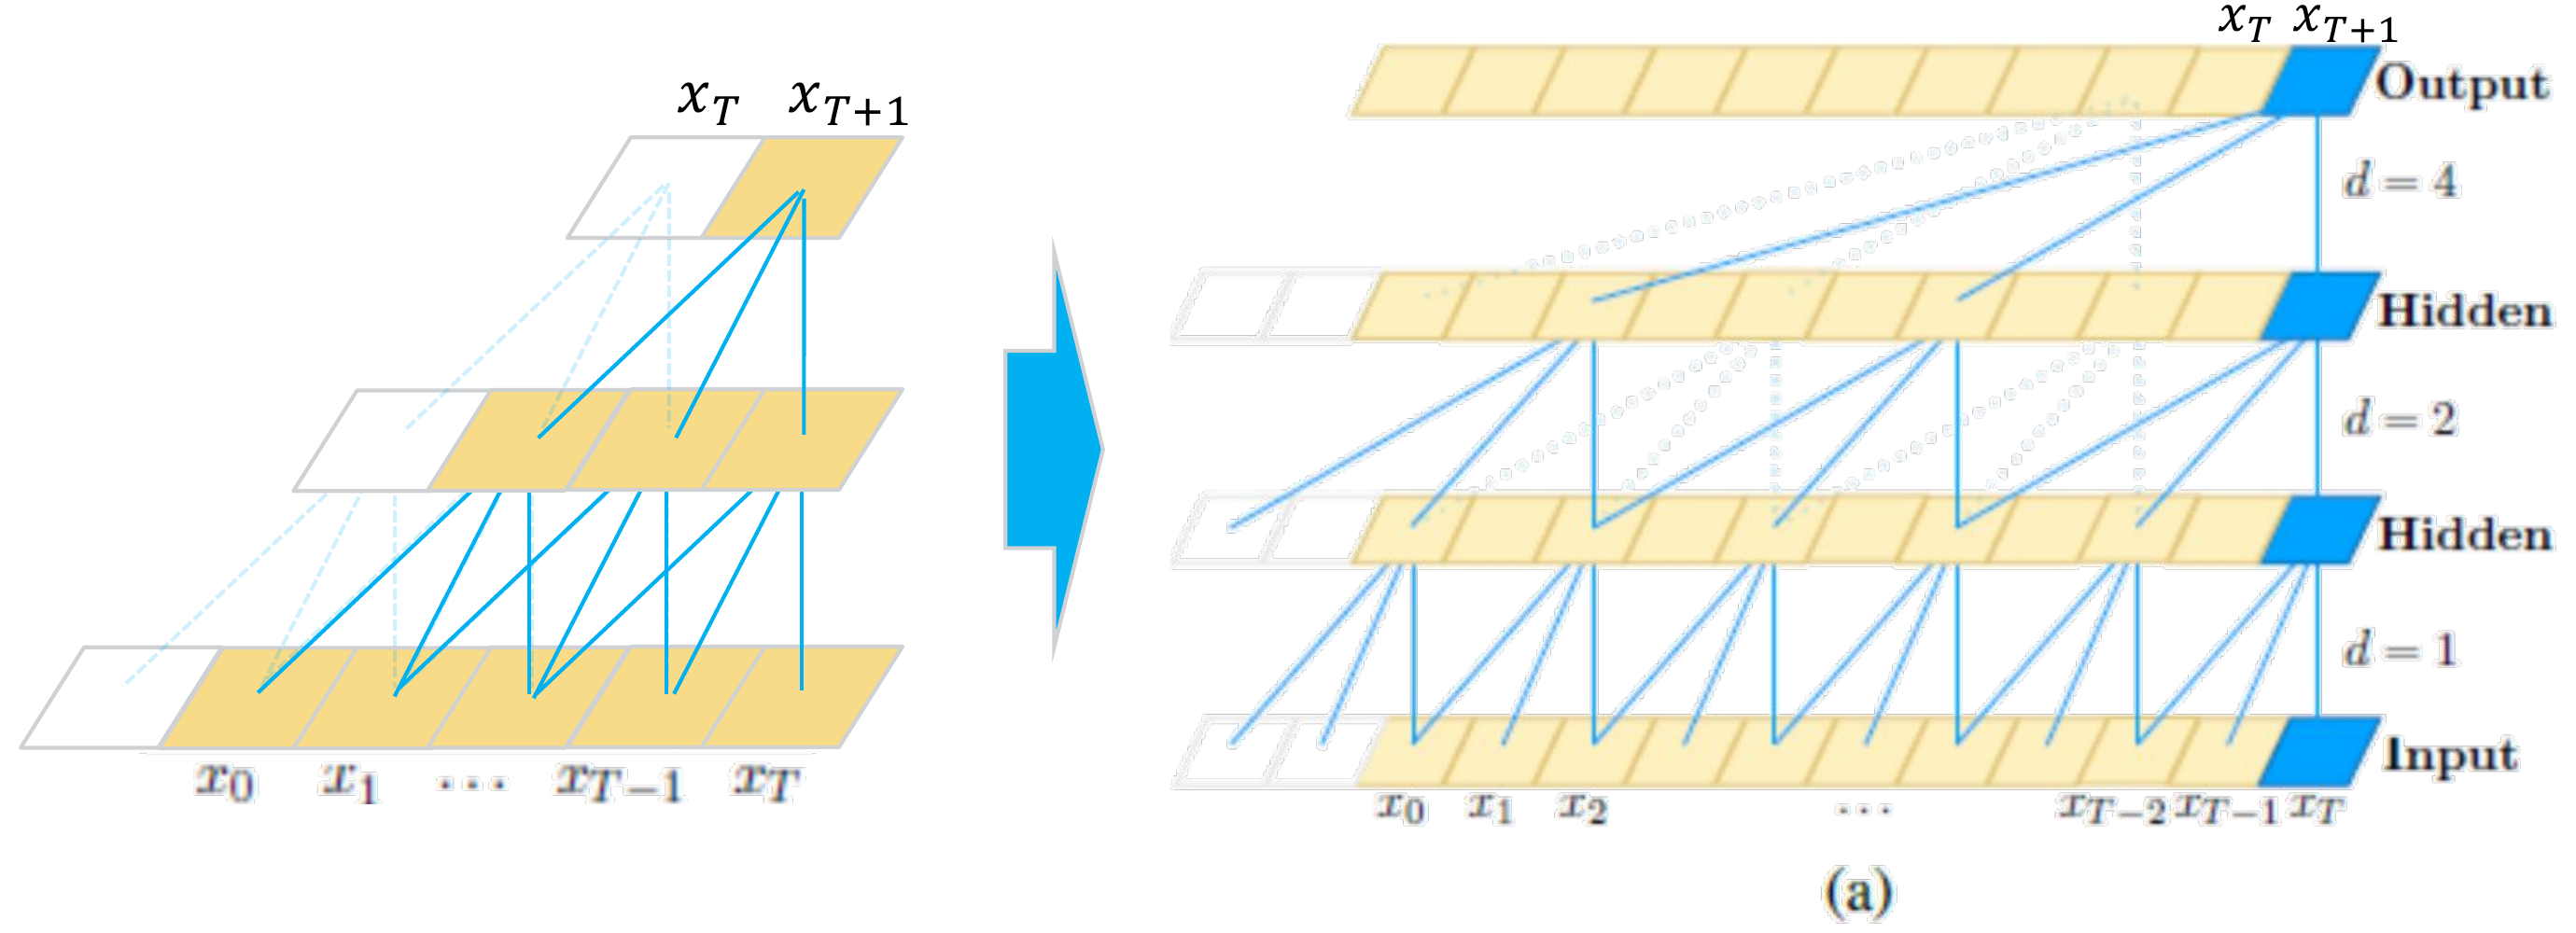
\includegraphics[width=0.92\textwidth]{Pictures/tcn_dilated.png}
    \caption{Architectural comparison between standard causal convolutions and dilated causal convolutions (Bai et al.~\cite{bai2018empirical}). Left: Standard causal convolution where receptive field grows linearly with depth. Right: Dilated causal convolution with exponentially doubling dilation factors ($d=1, 2, 4$), achieving exponential receptive field expansion without gaps in the input history.}\label{fig:tcn_dilated}
\end{figure}

\subsubsection{Comparative Architectural Analysis: Standard vs. Dilated Causal Convolutions}

Figure~\ref{fig:tcn_dilated} directly visualizes the paradigm shift from standard causal convolutions (left) to the dilated architecture proposed by Bai et al.~\cite{bai2018empirical} (right):

\begin{itemize}[leftmargin=*]
    \item \textbf{Left Panel --- Standard Causal Convolution (Linear Interaction Distance):}
    \begin{itemize}[nosep]
        \item \textit{Strict Causality:} Time flows from left to right ($x_0 \to x_1 \dots \to x_T$). Predictions evaluated at time $t$ must never access future observations ($x_{t+1}, x_{t+2}$). Consequently, the convolutional kernel is strictly causal: connections from upper layers descend exclusively vertically or diagonally towards the left (past), ensuring zero lookahead.
        \item \textit{The Receptive Field Bottleneck:} With a standard kernel size $K$ and no dilation ($d=1$), each additional layer increases the receptive field by only $K-1$ past time steps:
        \[ \text{Receptive Field} = 1 + L(K - 1) \]
        As visible in the narrow triangular pyramid on the left, capturing a historical horizon of $N$ time steps requires $L \approx N / (K - 1)$ layers. For long temporal sequences (e.g., $N = 1000$), an impractically deep network of hundreds of layers would be required, introducing severe computational costs and optimization difficulties.
    \end{itemize}

    \item \textbf{Right Panel --- Dilated Causal Convolution (Exponential Receptive Field):}
    Instead of growing the filter size or stacking hundreds of layers, the network keeps small, efficient kernels (e.g., $K=2$ parameters per channel) while exponentially doubling the dilation factor $d$ at each successive layer:
    \begin{enumerate}[nosep]
        \item \textbf{Input Layer (bottom):} Represents the raw discrete input sequence $(x_0, x_1, \dots, x_T)$.
        \item \textbf{First Hidden Layer ($d = 1$):} Standard stride-1 causal convolution. Each node aggregates 2 consecutive values ($x_t$ and $x_{t-1}$).
        \item \textbf{Second Hidden Layer ($d = 2$):} The dilation factor doubles to $d=2$. The filter spans 2 positions spaced by 2 time steps (sampling $t$ and $t-2$, skipping the intermediate point).
        \item \textbf{Output Layer ($d = 4$):} The dilation factor doubles again to $d=4$. The filter samples features spaced 4 time steps apart (at $t$ and $t-4$).
    \end{enumerate}

    \item \textbf{Tracing the Blue Receptive Tree (Top-Right Node at $x_T$):}
    Following the blue highlighted connections backwards in Figure~\ref{fig:tcn_dilated} illustrates how exponential dilation covers the past:
    \begin{itemize}[nosep]
        \item At layer $d=4$, the top-right output node branches into \textbf{2 features} (at $T$ and $T-4$).
        \item At layer $d=2$, each of these two features branches into 2 nodes at stride 2, yielding \textbf{4 features} ($T, T-2, T-4, T-6$).
        \item At layer $d=1$, each of these four features branches into 2 adjacent nodes, covering \textbf{8 consecutive input tokens} ($x_{T-7}, x_{T-6}, \dots, x_T$).
    \end{itemize}
    With only 3 convolutional layers and $K=2$, the receptive field spans 8 full time steps.
\end{itemize}

\begin{keywordbox}
\textbf{Why Dilation is Logarithmic and Continuous (w/o Gaps)} \\
\textbf{1. Logarithmic Depth Requirement:} Because the effective receptive span doubles with every layer ($1, 2, 4, 8, \dots$), the receptive field scales exponentially with depth:
\[ \text{Receptive Field} = 1 + (K - 1) \sum_{l=0}^{L-1} 2^l = 1 + (K - 1)(2^L - 1) \]
To observe a temporal context of length $N$, the required network depth scales \textbf{logarithmically}:
\[ L \approx \log_2(N) \]
For instance, while a standard causal convolution would require $\approx 1000$ layers to observe $1000$ historical steps, a dilated TCN achieves this with just $\lceil \log_2(1000) \rceil = 10$ layers!

\textbf{2. Coverage Without Gaps (\textit{w/o gaps}):} Although individual higher-level filters skip intermediate activations, the hierarchical doubling of dilation factors ($d_l = 2^l$) ensures that every single discrete input token within the receptive span contributes to the final prediction. There are no temporal holes or unobserved steps in the input history.
\end{keywordbox}

\subsection{Trade-offs of Temporal Convolutional Networks}

\begin{InsightBox}
\textbf{Advantages and Disadvantages of TCNs:}
\begin{itemize}[leftmargin=*]
    \item \textbf{Pros:}
    \begin{itemize}[nosep]
        \item \textbf{Parallelization:} Unlike recurrent architectures, convolutions can be computed concurrently across all time steps during training, drastically accelerating training times.
        \item \textbf{Local Dependencies:} Convolutions excel at modeling localized temporal features and patterns.
    \end{itemize}
    \item \textbf{Cons:}
    \begin{itemize}[nosep]
        \item \textbf{Fixed Maximum Memory:} The receptive field is strictly bounded by the network depth and dilation schedule; historical information beyond this window is permanently lost.
        \item \textbf{Inflexibility at Test Time:} Handling variable sequence lengths or streaming evaluation requires managing historical buffers, whereas recurrent models update a single internal state vector dynamically.
    \end{itemize}
\end{itemize}
\end{InsightBox}

\section{Recurrent Neural Networks}

The primary and historically dominant paradigm for processing sequential data is the \textbf{Recurrent Neural Network (RNN)}. Instead of relying on expanding spatial filters, an RNN introduces an internal \textbf{hidden state} that acts as a dynamic memory buffer.

\subsection{The Recurrence Principle}

At each time step $t$, the network processes an incoming input $x_t$ while retaining a memory vector of past computations, denoted as the \textbf{hidden state} $h_{t-1}$. The state is updated via a recurrence formula:

\begin{equation}
h_t = f_W(h_{t-1}, x_t)
\label{eq:rnn_general}
\end{equation}

When output predictions are required, the current hidden state is mapped to an output vector:

\begin{equation}
y_t = f_{W_{hy}}(h_t)
\label{eq:rnn_output}
\end{equation}

\begin{Notebox}
\textbf{Piece-by-Piece Breakdown of Equations~\ref{eq:rnn_general} and~\ref{eq:rnn_output}:}
\begin{itemize}[nosep, leftmargin=*]
    \item $t$: The current discrete time step index ($t = 1, 2, \dots, T$).
    \item $h_t$: The \textbf{new hidden state} vector at time $t$, capturing the historical context up to the current moment.
    \item $h_{t-1}$: The \textbf{previous hidden state} vector from time step $t-1$ (with $h_0$ typically initialized to zero).
    \item $x_t$: The \textbf{input vector} fed into the network at time step $t$.
    \item $f_W$: A parameterized non-linear state transition function. \textbf{Crucial property:} \textit{the exact same function $f_W$ and the exact same set of parameters $W$ are reused identically across every time step}.
    \item $y_t$: The predicted output vector (e.g., class logits) generated at time step $t$.
    \item $f_{W_{hy}}$: The output mapping function parameterized by weights $W_{hy}$.
\end{itemize}
\end{Notebox}

\subsection{The Vanilla RNN Formulation}

In the classic formulation (often called the \textbf{Vanilla RNN} or \textbf{Elman RNN}), the transition function applies affine transformations followed by a hyperbolic tangent ($\tanh$) non-linearity:

\begin{equation}
h_t = \tanh(W_{hh} h_{t-1} + W_{xh} x_t)
\label{eq:vanilla_rnn_state}
\end{equation}

\begin{equation}
y_t = W_{hy} h_t
\label{eq:vanilla_rnn_out}
\end{equation}

\begin{Notebox}
\textbf{Piece-by-Piece Mathematical Breakdown of Equation~\ref{eq:vanilla_rnn_state}:}
\begin{itemize}[nosep, leftmargin=*]
    \item $W_{hh}$: The \textbf{hidden-to-hidden weight matrix}. It transforms the previous memory vector $h_{t-1}$, governing how historical context propagates into the future.
    \item $W_{xh}$: The \textbf{input-to-hidden weight matrix}. It projects the incoming input vector $x_t$ into the hidden feature space.
    \item $\tanh$: The hyperbolic tangent activation function. It squashes state values strictly into the interval $(-1, 1)$, preventing activations from growing unbounded across successive steps.
    \item $W_{hy}$: The \textbf{hidden-to-output weight matrix}. It projects the internal hidden representation $h_t$ into the target output space.
\end{itemize}
\end{Notebox}

\subsection{Unrolling the Computational Graph}

To understand how an RNN is trained, the recurrence is unrolled across time into a directed acyclic computational graph, as shown in Figure~\ref{fig:rnn_unrolled}.

\begin{figure}[htbp]
    \centering
    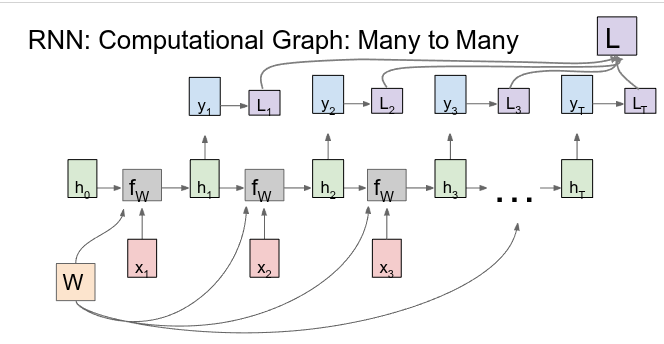
\includegraphics[width=0.85\textwidth]{Pictures/rnn_unrolled.png}
    \caption{Unrolled computational graph of a recurrent neural network across time steps $t=1, \dots, T$. Notice that the weight matrix $W$ is reused identically at every time step.}\label{fig:rnn_unrolled}
\end{figure}

At each time step $t$, the network receives input $x_t$, updates its hidden state $h_t$, and optionally emits an output $y_t$. If a target label $y_t^*$ is available, a local loss $L_t$ is computed. The total loss across the full sequence of length $T$ is the accumulated sum:
\[ L = \sum_{t=1}^T L_t \]

\subsection{Sequence-to-Sequence: Synchronized vs. Encoder-Decoder Mappings}

When modeling sequences with inputs and outputs, two distinct structural paradigms emerge from the computational graph, as introduced in the lecture slides (Slides 41--46):

\subsubsection{Synchronized Many-to-Many (Slide 41)}
In a synchronized recurrence, the network ingests an input $x_t$ and immediately emits a corresponding output $y_t$ at every time step $t$. While effective for tasks with strict 1:1 temporal alignment (e.g., frame-level video classification or part-of-speech tagging), this architecture fundamentally fails for tasks such as \textbf{Machine Translation}:
\begin{itemize}[nosep, leftmargin=*]
    \item \textbf{Length Disparity ($T_{\text{in}} \neq T_{\text{out}}$):} Natural languages rarely have matching word counts (e.g., English \textit{``I am hungry''} [3 words] $\longrightarrow$ Italian \textit{``Ho fame''} [2 words]). Synchronous evaluation cannot handle length discrepancies.
    \item \textbf{Structural Word Reordering:} Grammar and syntax vary across languages. In English, adjectives precede nouns (\textit{``the black cat''}), whereas in Italian they follow (\textit{``il gatto nero''}). A synchronized network would be forced to predict the first translated word before even observing the subsequent subject.
\end{itemize}

\subsubsection{Sequence-to-Sequence: Many-to-One + One-to-Many (Slides 45--46)}
To resolve these limitations, Sutskever et al.~\cite{sutskever2014sequence} (and Cho et al.~\cite{cho2014learning}) proposed the \textbf{Sequence-to-Sequence (Seq2Seq)} framework, decomposing the task into two decoupled recurrent modules operating in cascade, illustrated in Figure~\ref{fig:seq2seq_arch}:

\begin{figure}[htbp]
    \centering
    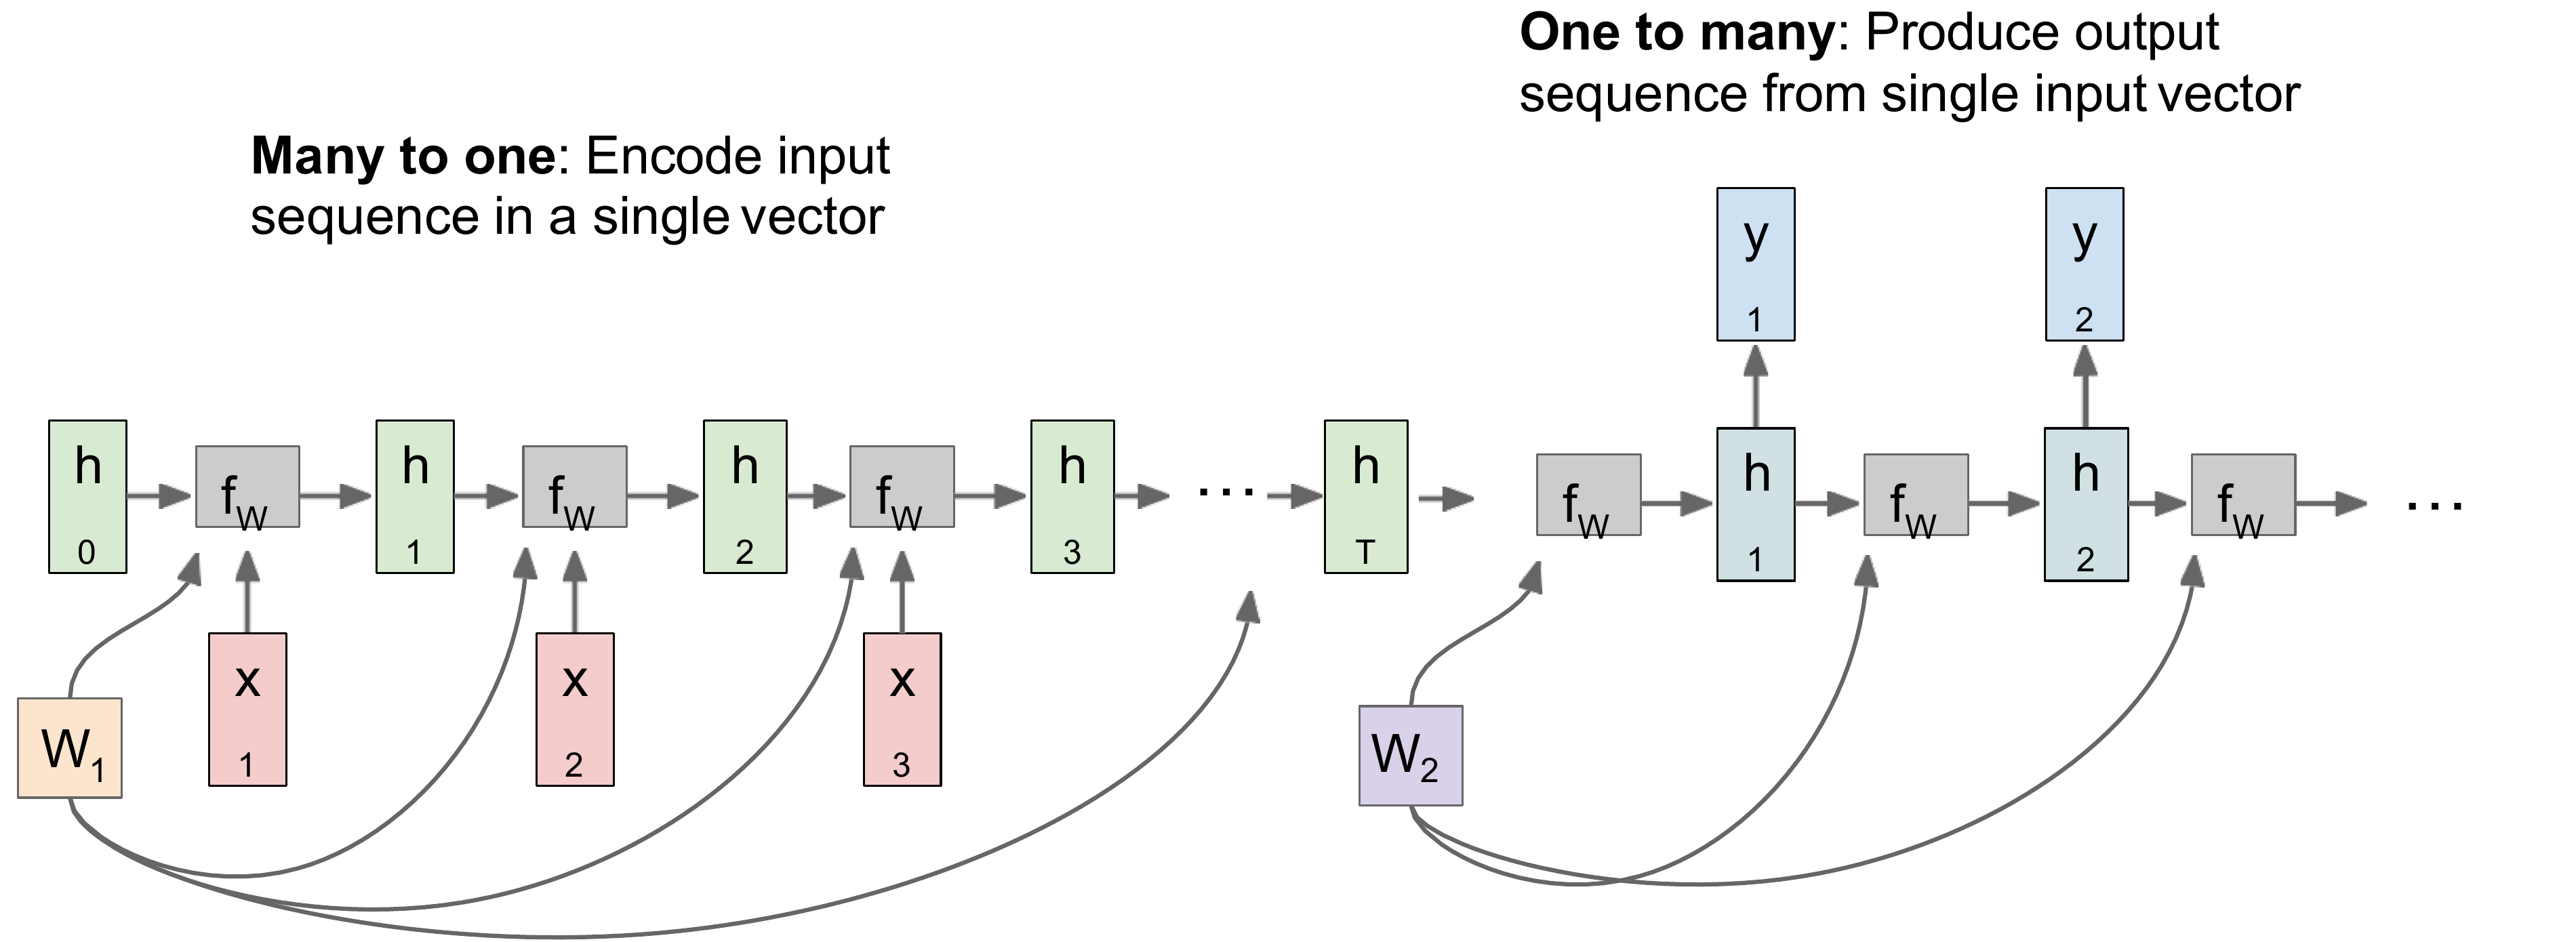
\includegraphics[width=0.92\textwidth]{Pictures/seq2seq_architecture.png}
    \caption{Sequence-to-Sequence architecture (Sutskever et al.~\cite{sutskever2014sequence}, from course slides). The Encoder (Many-to-One with weights $W_1$) compresses the source sequence into bottleneck state $h_T$. The Decoder (One-to-Many with weights $W_2$) generates the target sequence from $h_T$ until an end-of-sequence token is emitted.}\label{fig:seq2seq_arch}
\end{figure}

\begin{enumerate}[leftmargin=*]
    \item \textbf{Encoder --- Many-to-One (Parameterized by $W_1$):} \\
    The encoder consumes the entire input sequence $x_1, \dots, x_T$ step-by-step without producing intermediate outputs. Its sole purpose is to accumulate the full contextual meaning of the input into the final hidden state vector $h_T$, known as the \textbf{context} or \textbf{bottleneck vector}.
    \item \textbf{Decoder --- One-to-Many (Parameterized by $W_2$):} \\
    The decoder receives $h_T$ as its initial hidden state and autoregressively generates the output sequence $y_1, y_2, \dots, y_{T'}$. Generation terminates dynamically when the model emits an end-of-sequence token $\langle\text{END}\rangle$, allowing $T'$ to differ arbitrarily from $T$.
\end{enumerate}

\begin{keywordbox}
\textbf{Why Two Distinct Weight Sets ($W_1 \neq W_2$)?} \\
The encoder weights $W_1$ and decoder weights $W_2$ are explicitly decoupled:
\begin{itemize}[nosep, leftmargin=*]
    \item $W_1$ learns temporal dynamics, grammar, and semantic representations of the \textbf{source} domain (e.g., parsing English syntax).
    \item $W_2$ learns the vocabulary distributions, syntax rules, and generation dynamics of the \textbf{target} domain (e.g., generating fluent Italian sentences).
\end{itemize}
\end{keywordbox}

\subsection{Case Study: Character-Level Language Modeling}

To see an RNN in action, consider a character-level language model trained to predict the sequence \textit{``hello''} from a vocabulary of four letters: $\{h, e, l, o\}$ (Slides 47--53; Karpathy~\cite{karpathy2015unreasonable}). At each step, the network receives the current character and predicts a probability distribution over the vocabulary for the next character.

\subsubsection{Training Phase: Teacher Forcing}

During training, the complete sequence \textit{``hello''} is known in advance. The model is trained using \textbf{Teacher Forcing} (also called \textit{Ground Truth Forcing}), illustrated in Figure~\ref{fig:rnn_char_train}.

\begin{figure}[htbp]
    \centering
    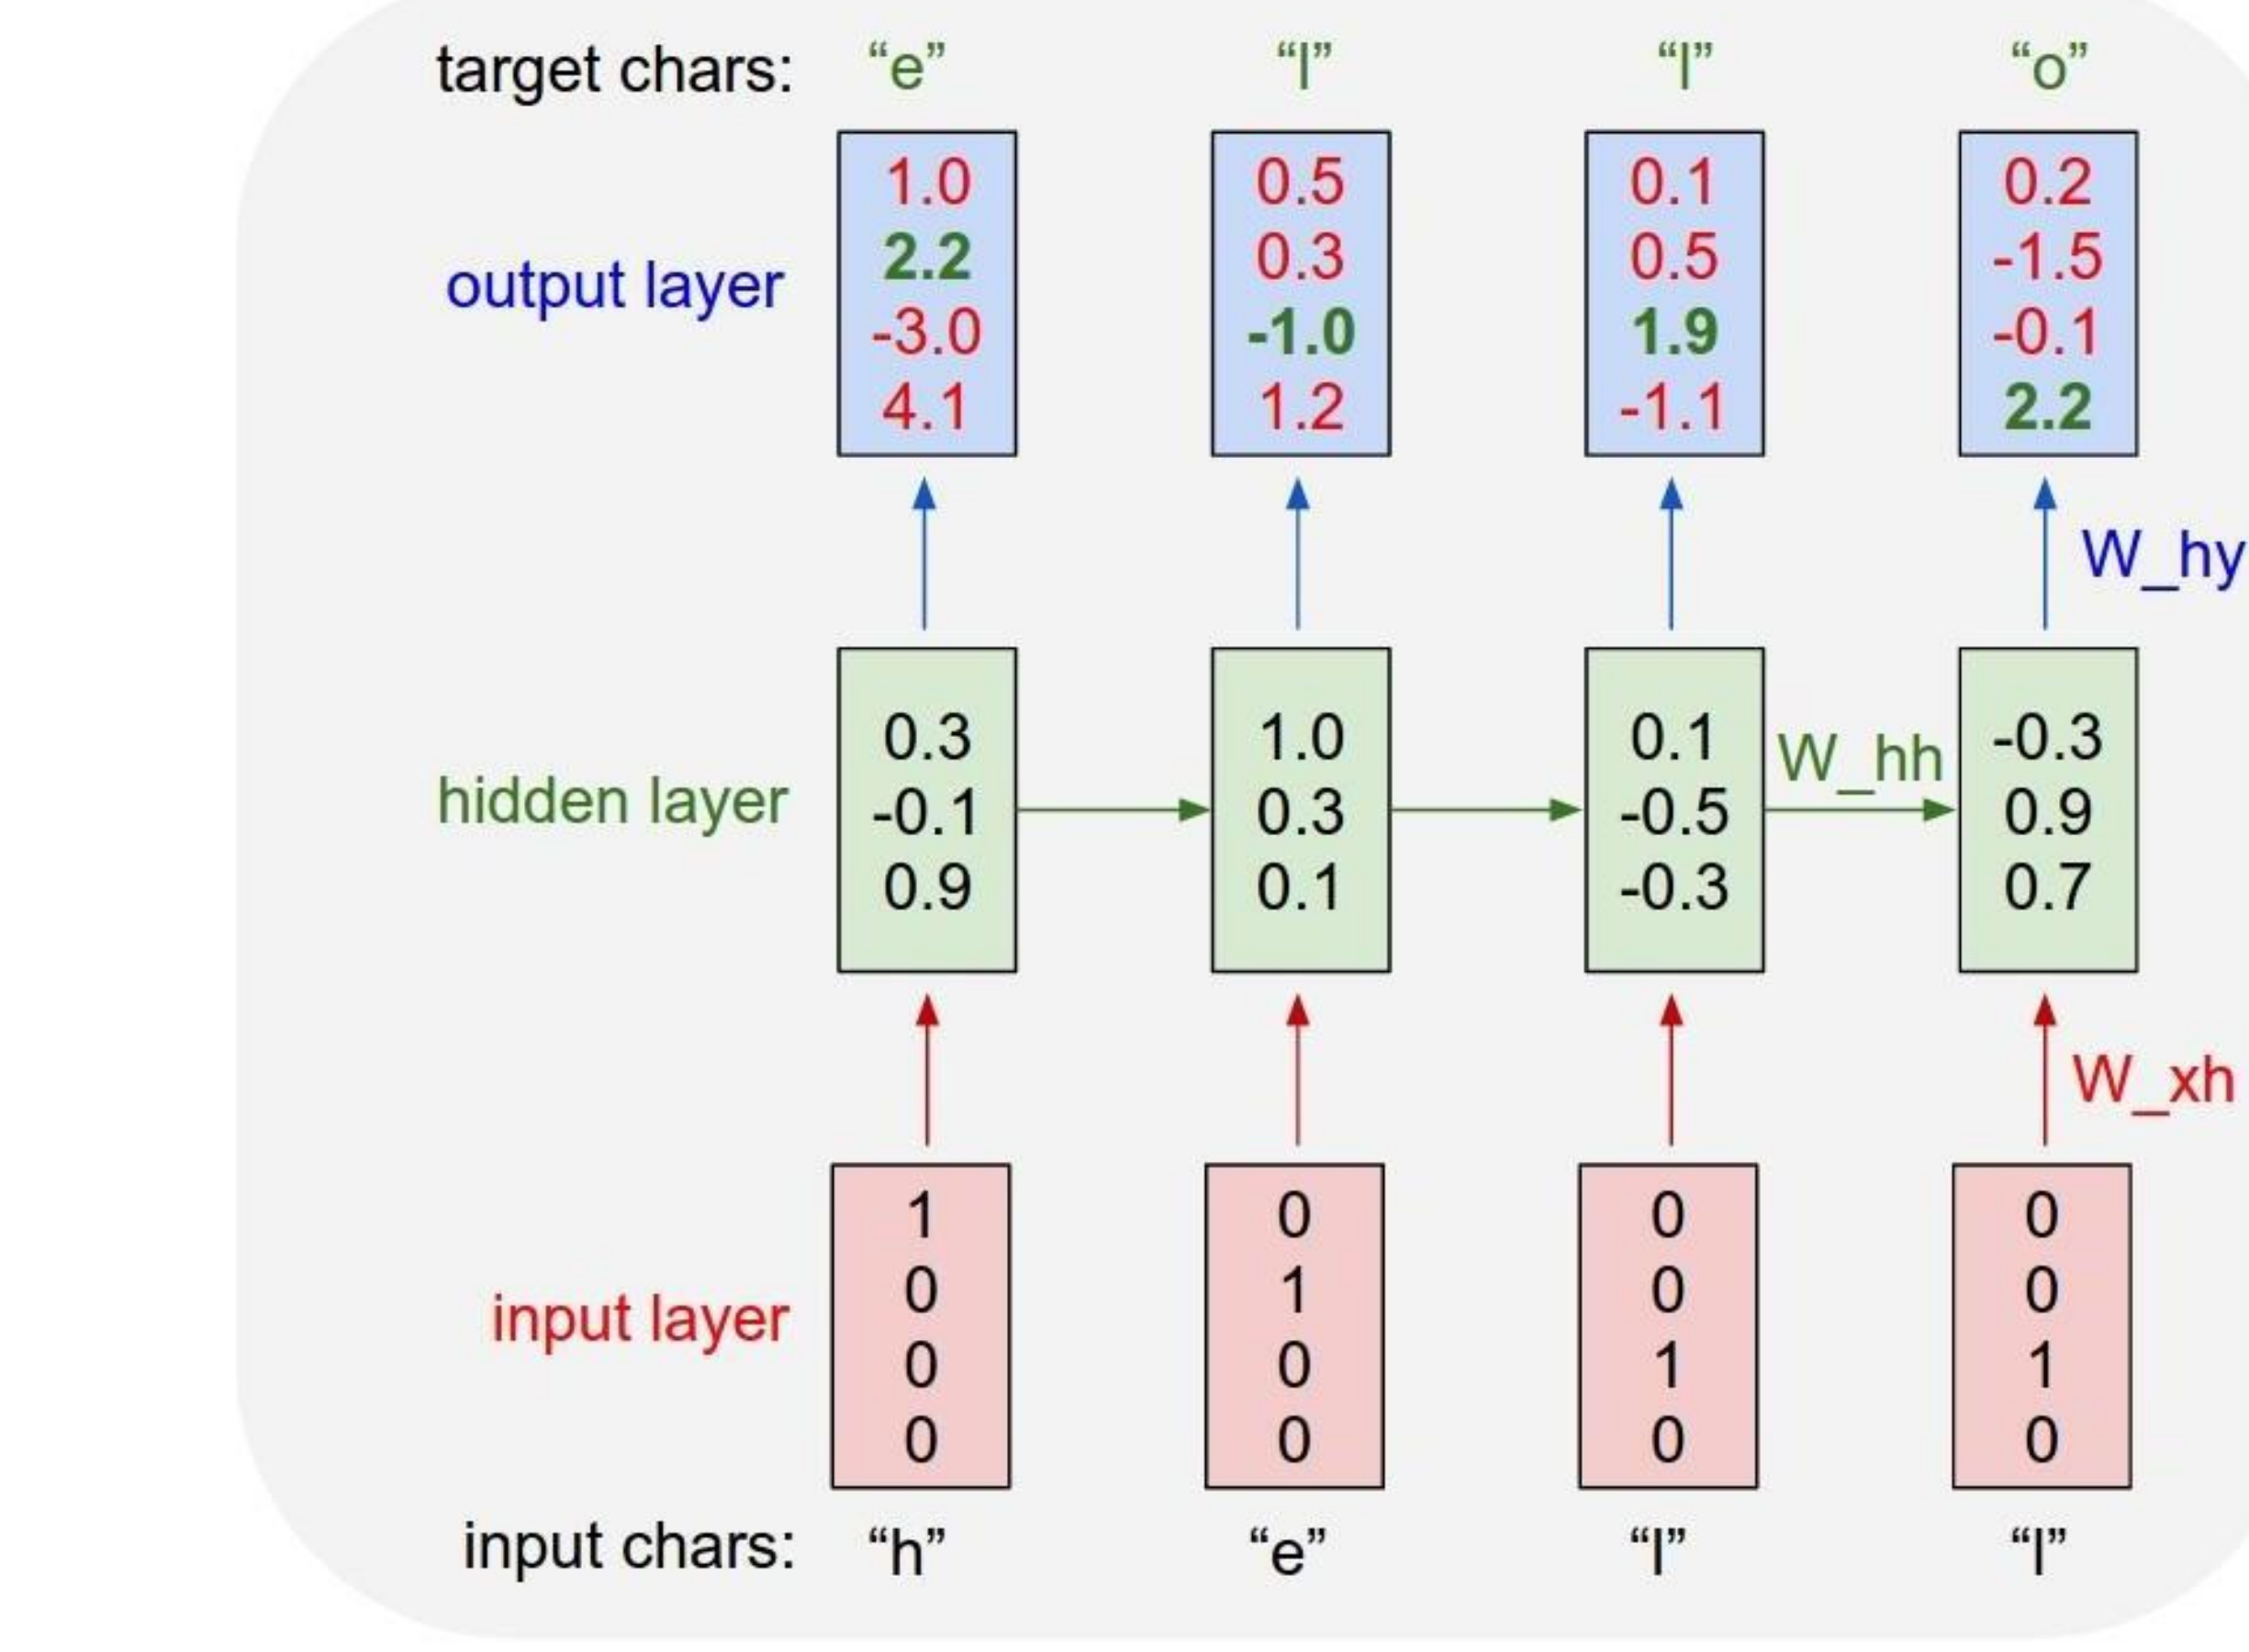
\includegraphics[width=0.68\textwidth]{Pictures/rnn_char_train.png}
    \caption{Training phase of the character-level RNN with Teacher Forcing (Slide 49). At each step, the ground-truth character from the dataset is fed as input, regardless of what the network predicted at the previous step.}\label{fig:rnn_char_train}
\end{figure}

As shown in Figure~\ref{fig:rnn_char_train}:
\begin{itemize}[leftmargin=*]
    \item \textbf{Network Flow:} Each character is represented as a one-hot vector in the input layer (4 red nodes), processed by the recurrent hidden layer (3 green nodes), and projected to raw scores (logits) in the output layer (4 blue nodes).
    \item \textbf{Teacher Forcing:} At each step $t$, the input is strictly the ground-truth character from the target word:
    \begin{itemize}[nosep]
        \item Feed \textit{`h'} $\longrightarrow$ target is \textit{`e'}
        \item Feed \textit{`e'} $\longrightarrow$ target is \textit{`l'}
        \item Feed \textit{`l'} $\longrightarrow$ target is \textit{`l'}
        \item Feed \textit{`l'} $\longrightarrow$ target is \textit{`o'}
    \end{itemize}
    Even if the network makes an incorrect prediction at step 1, step 2 is still fed the true character \textit{`e'}. This prevents errors from accumulating during training.
    \item \textbf{Memory Disambiguates Consecutive Letters:} Notice steps 3 and 4: both receive the identical input vector for \textit{`l'}, but step 3 must predict \textit{`l'} while step 4 must predict \textit{`o'}. A static feedforward network cannot tell them apart. The RNN succeeds because its hidden state acts as memory: step 3 remembers the past context $[h \to e \to l]$, whereas step 4 remembers $[h \to e \to l \to l]$.
\end{itemize}

\subsubsection{Test Phase: Autoregressive Generation}

At test time, the model must generate text autonomously without ground-truth answers. It operates in an \textbf{Autoregressive Loop}, shown in Figure~\ref{fig:rnn_char_test}.

\begin{figure}[htbp]
    \centering
    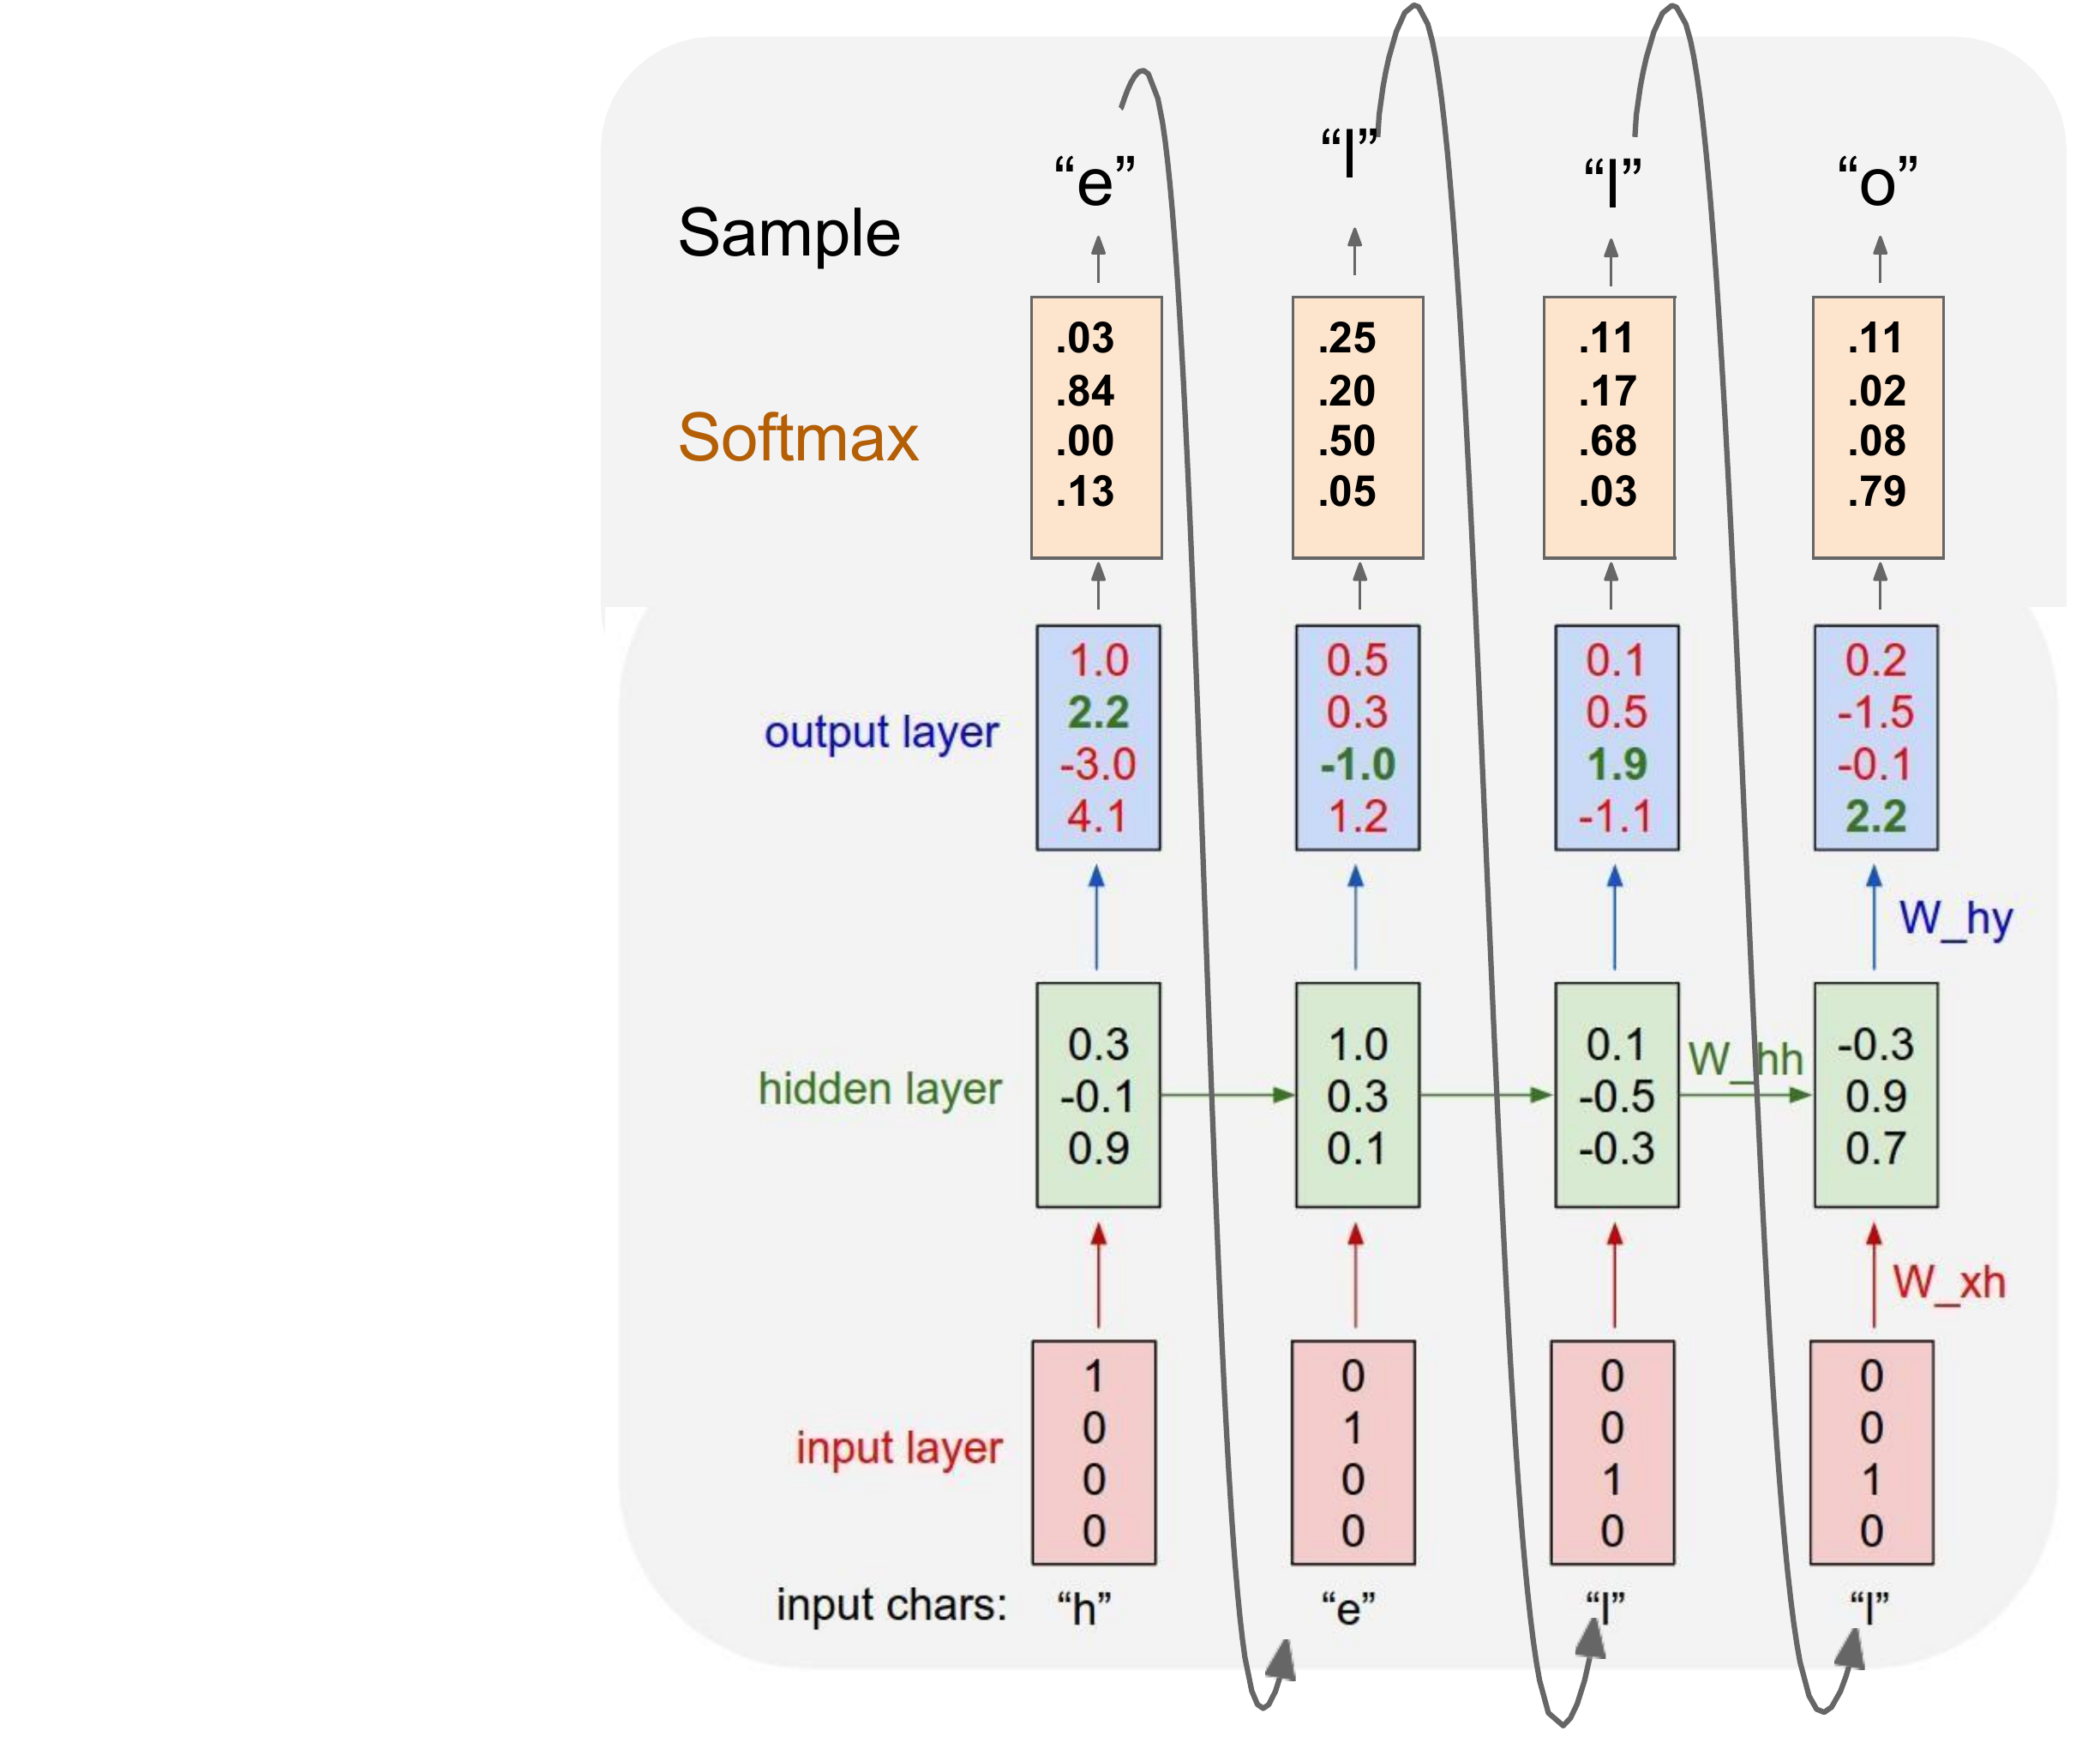
\includegraphics[width=0.68\textwidth]{Pictures/rnn_char_test.png}
    \caption{Test phase of the character-level RNN (Slide 53). Characters sampled from the output distribution are fed back recursively as inputs for the next time step (curved loop arrows).}\label{fig:rnn_char_test}
\end{figure}

The generation proceeds step by step:
\begin{itemize}[leftmargin=*]
    \item \textbf{Recursive Feedback:} Because there is no teacher at test time, the character produced at step $t$ is fed back as the input for step $t+1$, as traced by the curved arrows in Figure~\ref{fig:rnn_char_test}.
    \item \textbf{Sampling from Softmax:}
    \begin{enumerate}[nosep]
        \item \textbf{Seed Prompt ($t=1$):} We provide an initial character, $x_1 = \text{\textit{`h'}}$. The network computes output scores and converts them to probabilities via Softmax (yielding $P(e) = 0.84$). We sample token \textit{`e'}.
        \item \textbf{Step $t=2$:} The sampled \textit{`e'} is fed back as input $x_2$. Combining it with the internal hidden state, the network predicts probabilities and samples \textit{`l'} ($P(l) = 0.50$).
        \item \textbf{Step $t=3$:} The sampled \textit{`l'} is fed back as input $x_3$, yielding another sampled \textit{`l'} ($P(l) = 0.68$).
        \item \textbf{Step $t=4$:} The second \textit{`l'} is fed back as input $x_4$. Thanks to the internal memory accumulated over time, the network recognizes the completed prefix and samples \textit{`o'} ($P(o) = 0.79$).
    \end{enumerate}
\end{itemize}

\begin{keywordbox}
\textbf{Training vs. Testing at a Glance}\par\vspace{0.3em}
\begin{itemize}[nosep, leftmargin=*]
    \item \textbf{Training (Teacher Forcing):} Inputs come from the real dataset. Errors do not compound because the ground truth is provided at every step.
    \item \textbf{Testing (Autoregressive):} Inputs come from the model's own previous outputs. The network generates sequences recursively on its own.
\end{itemize}
\end{keywordbox}

\subsection{Case Study: Image Captioning (CNN + RNN)}

Another foundational application of recurrent models is \textbf{Image Captioning} (Slides 112--123, pioneered by Vinyals et al.~\cite{vinyals2015show}, Karpathy and Fei-Fei~\cite{karpathy2015deep}, and Donahue et al.~\cite{donahue2015long}): given an input image, the network must generate a fluent sentence describing its visual content. This represents a canonical \textbf{One-to-Many} task that unifies Computer Vision (CNN) and Natural Language Processing (RNN).

\subsubsection{How CNN and RNN Interact}

The architecture combines a Convolutional Neural Network (as a visual feature extractor) and a Recurrent Neural Network (as a sequential language generator), as shown in Figure~\ref{fig:captioning_interaction}.

\begin{figure}[htbp]
    \centering
    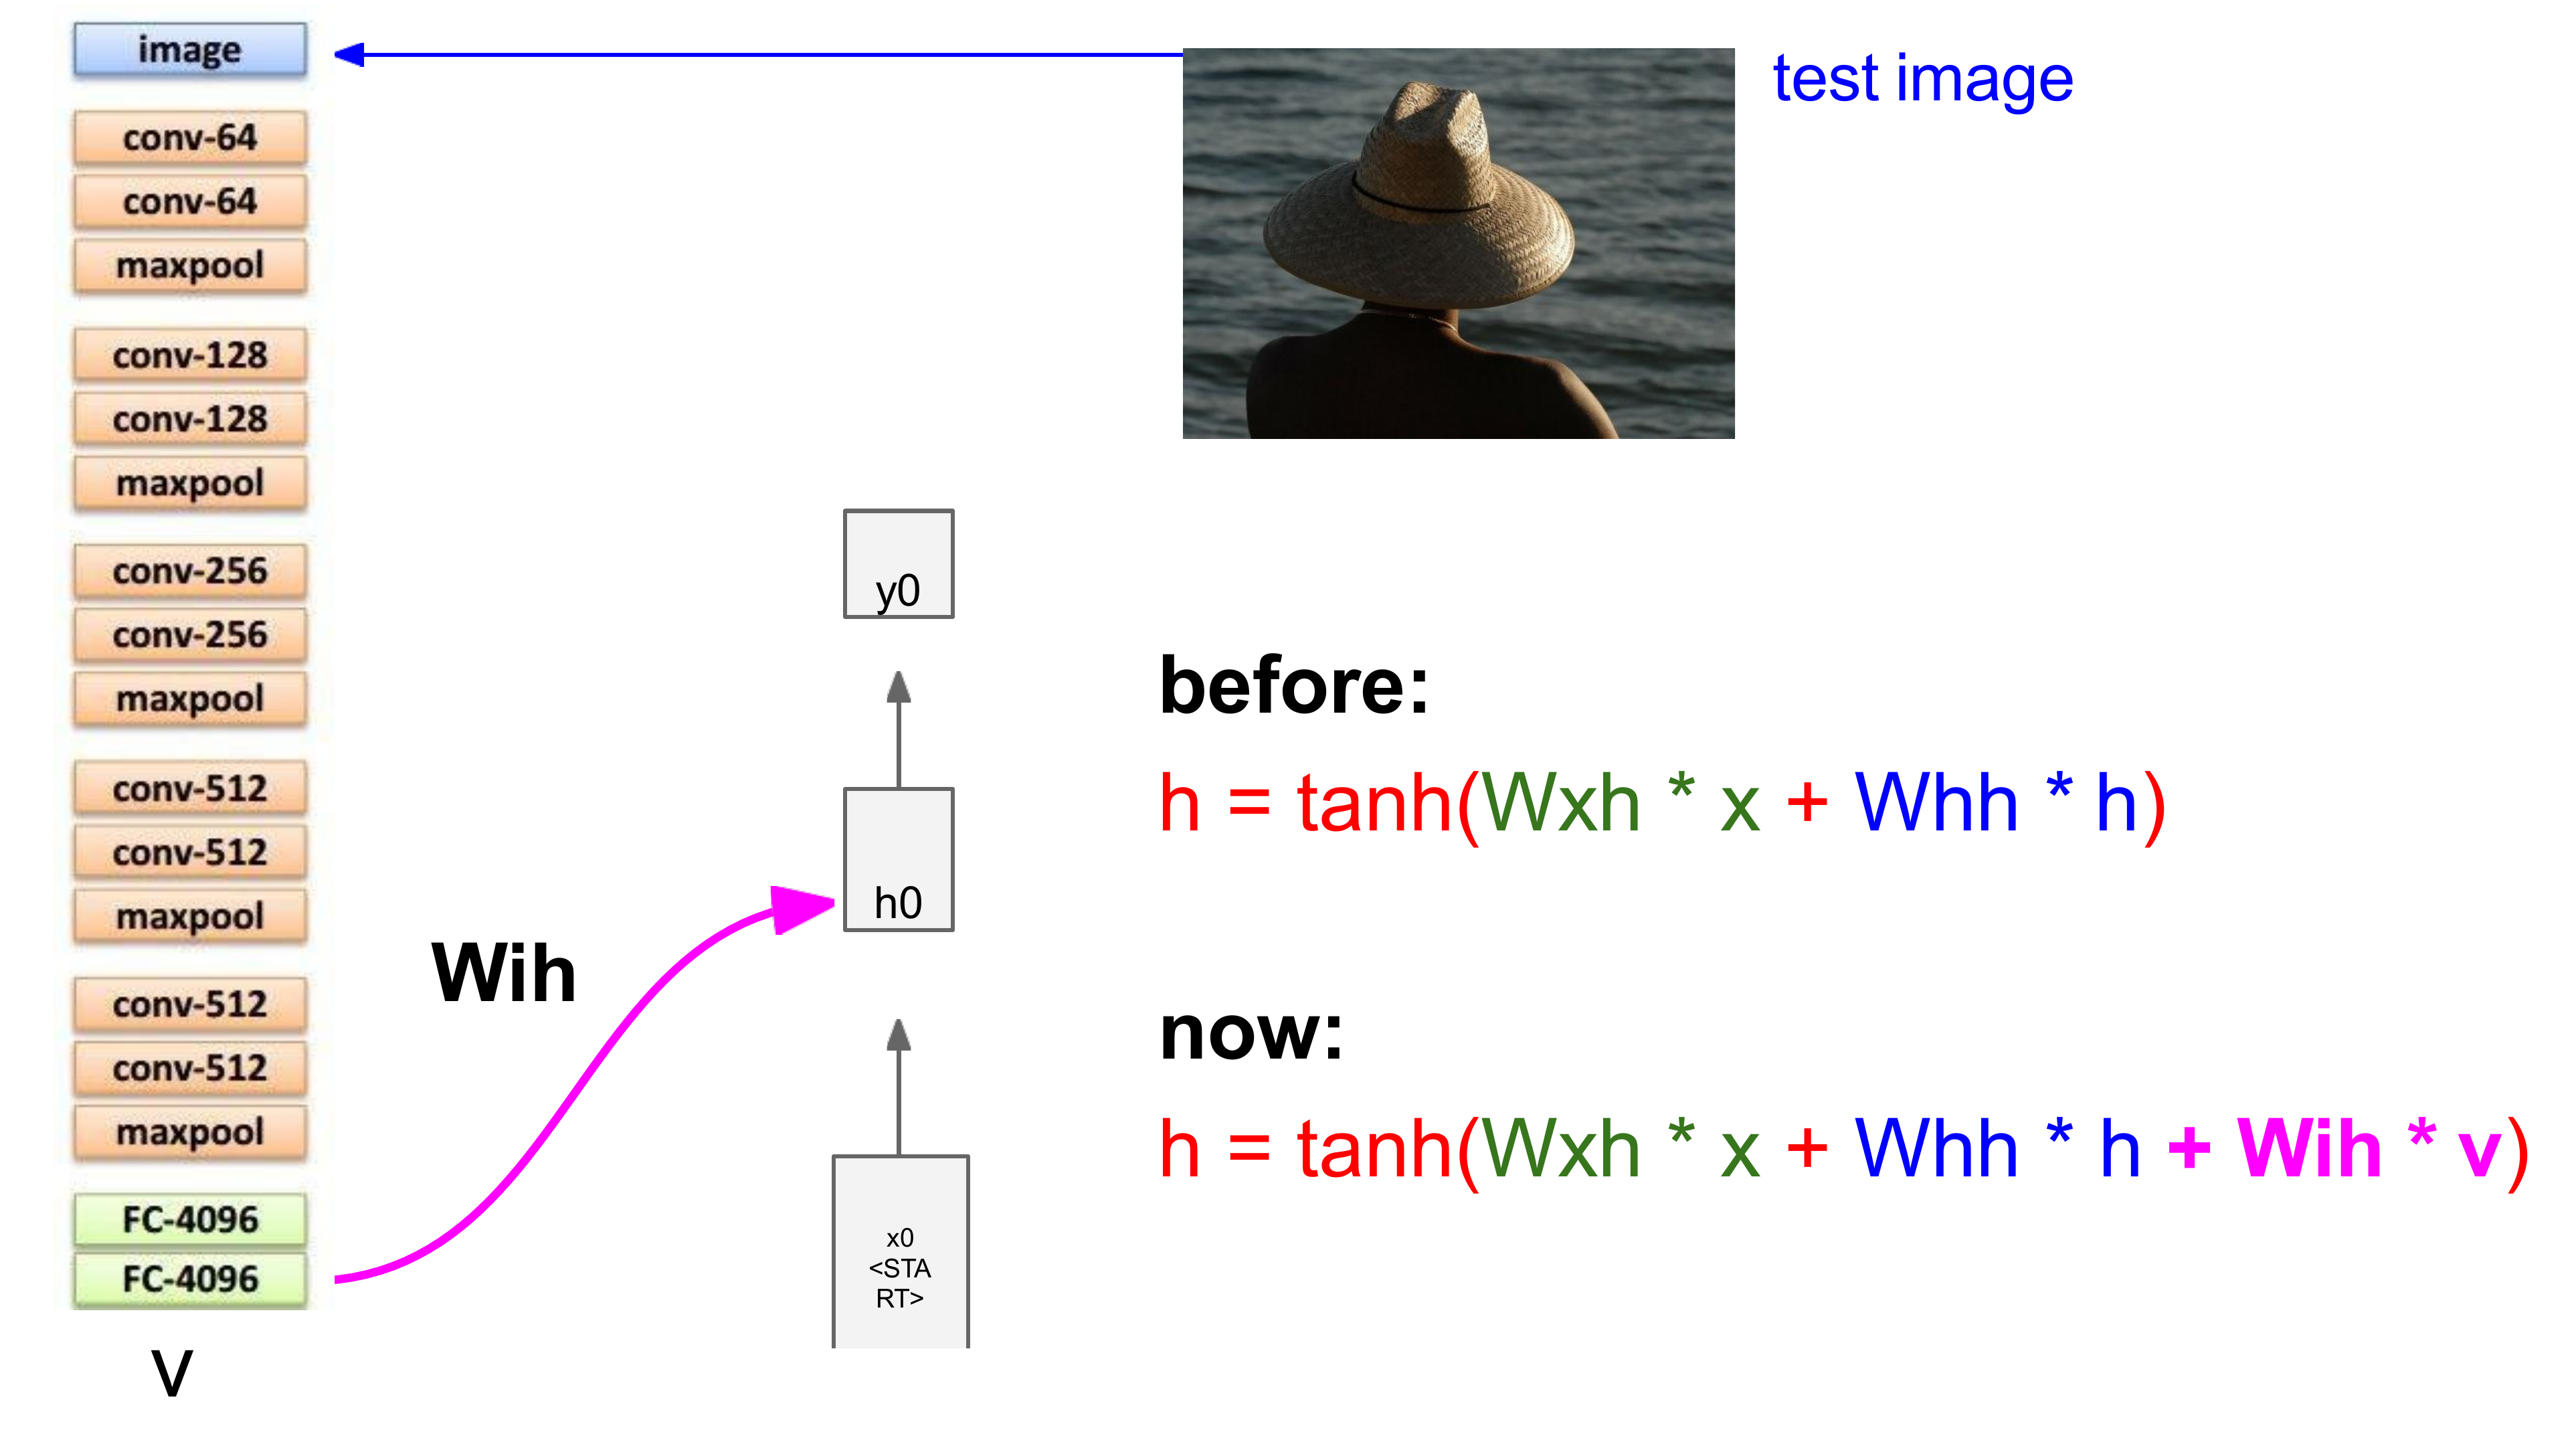
\includegraphics[width=0.54\textwidth]{Pictures/image_captioning_interaction.png}
    \caption{Interaction between CNN and RNN for Image Captioning (Slide 118). The CNN extracts visual feature vector $v$ from a pre-trained layer, which is injected into the RNN recurrence via weight matrix $W_{ih}$.}\label{fig:captioning_interaction}
\end{figure}

The interaction between the two networks proceeds as follows:
\begin{itemize}[leftmargin=*]
    \item \textbf{Visual Feature Extraction (CNN):} The input image is fed into a convolutional network (such as a pre-trained VGG-16). Crucially, the final classification layer (which predicts ImageNet class scores with Softmax) is discarded. Instead, we extract the dense feature vector $v \in \mathbb{R}^{4096}$ from the penultimate fully connected layer (\texttt{FC-4096}), capturing the global semantic content of the image.
    \item \textbf{The Recurrence Equation (Slide 118):} While a standard RNN computes $h_t = \tanh(W_{xh} x_t + W_{hh} h_{t-1})$, in Image Captioning the visual feature vector $v$ is added as a dedicated third input term:
    \[ h_t = \tanh(W_{xh} x_t + W_{hh} h_{t-1} + W_{ih} v) \]
\end{itemize}

\begin{Notebox}
    \textbf{What Learns vs. What Remembers (Parameters vs. Context):}
    \begin{itemize}[nosep]
        \item \textbf{The Learnable Weights (What changes during training):} The matrices $W_{xh}$, $W_{hh}$, $W_{ih}$ (alongside output projection $W_{hy}$) are the actual parameters of the model. During training via BPTT, backpropagation updates \textbf{only these weight matrices}. They learn the optimal transition rules: how to interpret words, how to advance memory, and how to project image features. At test time, all $W$ matrices are frozen.
        \item \textbf{The Hidden State ($h_t$):} The hidden state does \textbf{not} contain learnable weights. It is an activation vector acting as temporary working memory (functioning like a continuous Markovian state) that compresses the visual context $v$ and the sequence of words generated so far. It updates dynamically at every time step and resets to $\vec{0}$ for each new image.
        \item \textbf{The Inputs ($x_t$ and $v$):} Vector $v$ is the static visual embedding anchoring the language to the image, while $x_t$ is the text input ($x_0 = \texttt{<START>}$ at $t=0$, followed by the word sampled at step $t-1$).
    \end{itemize}
\end{Notebox}

\subsubsection{Autoregressive Caption Generation}

At inference time, the unrolled RNN generates the descriptive sentence word by word, as illustrated in Figure~\ref{fig:captioning_unrolled}.

\begin{figure}[htbp]
    \centering
    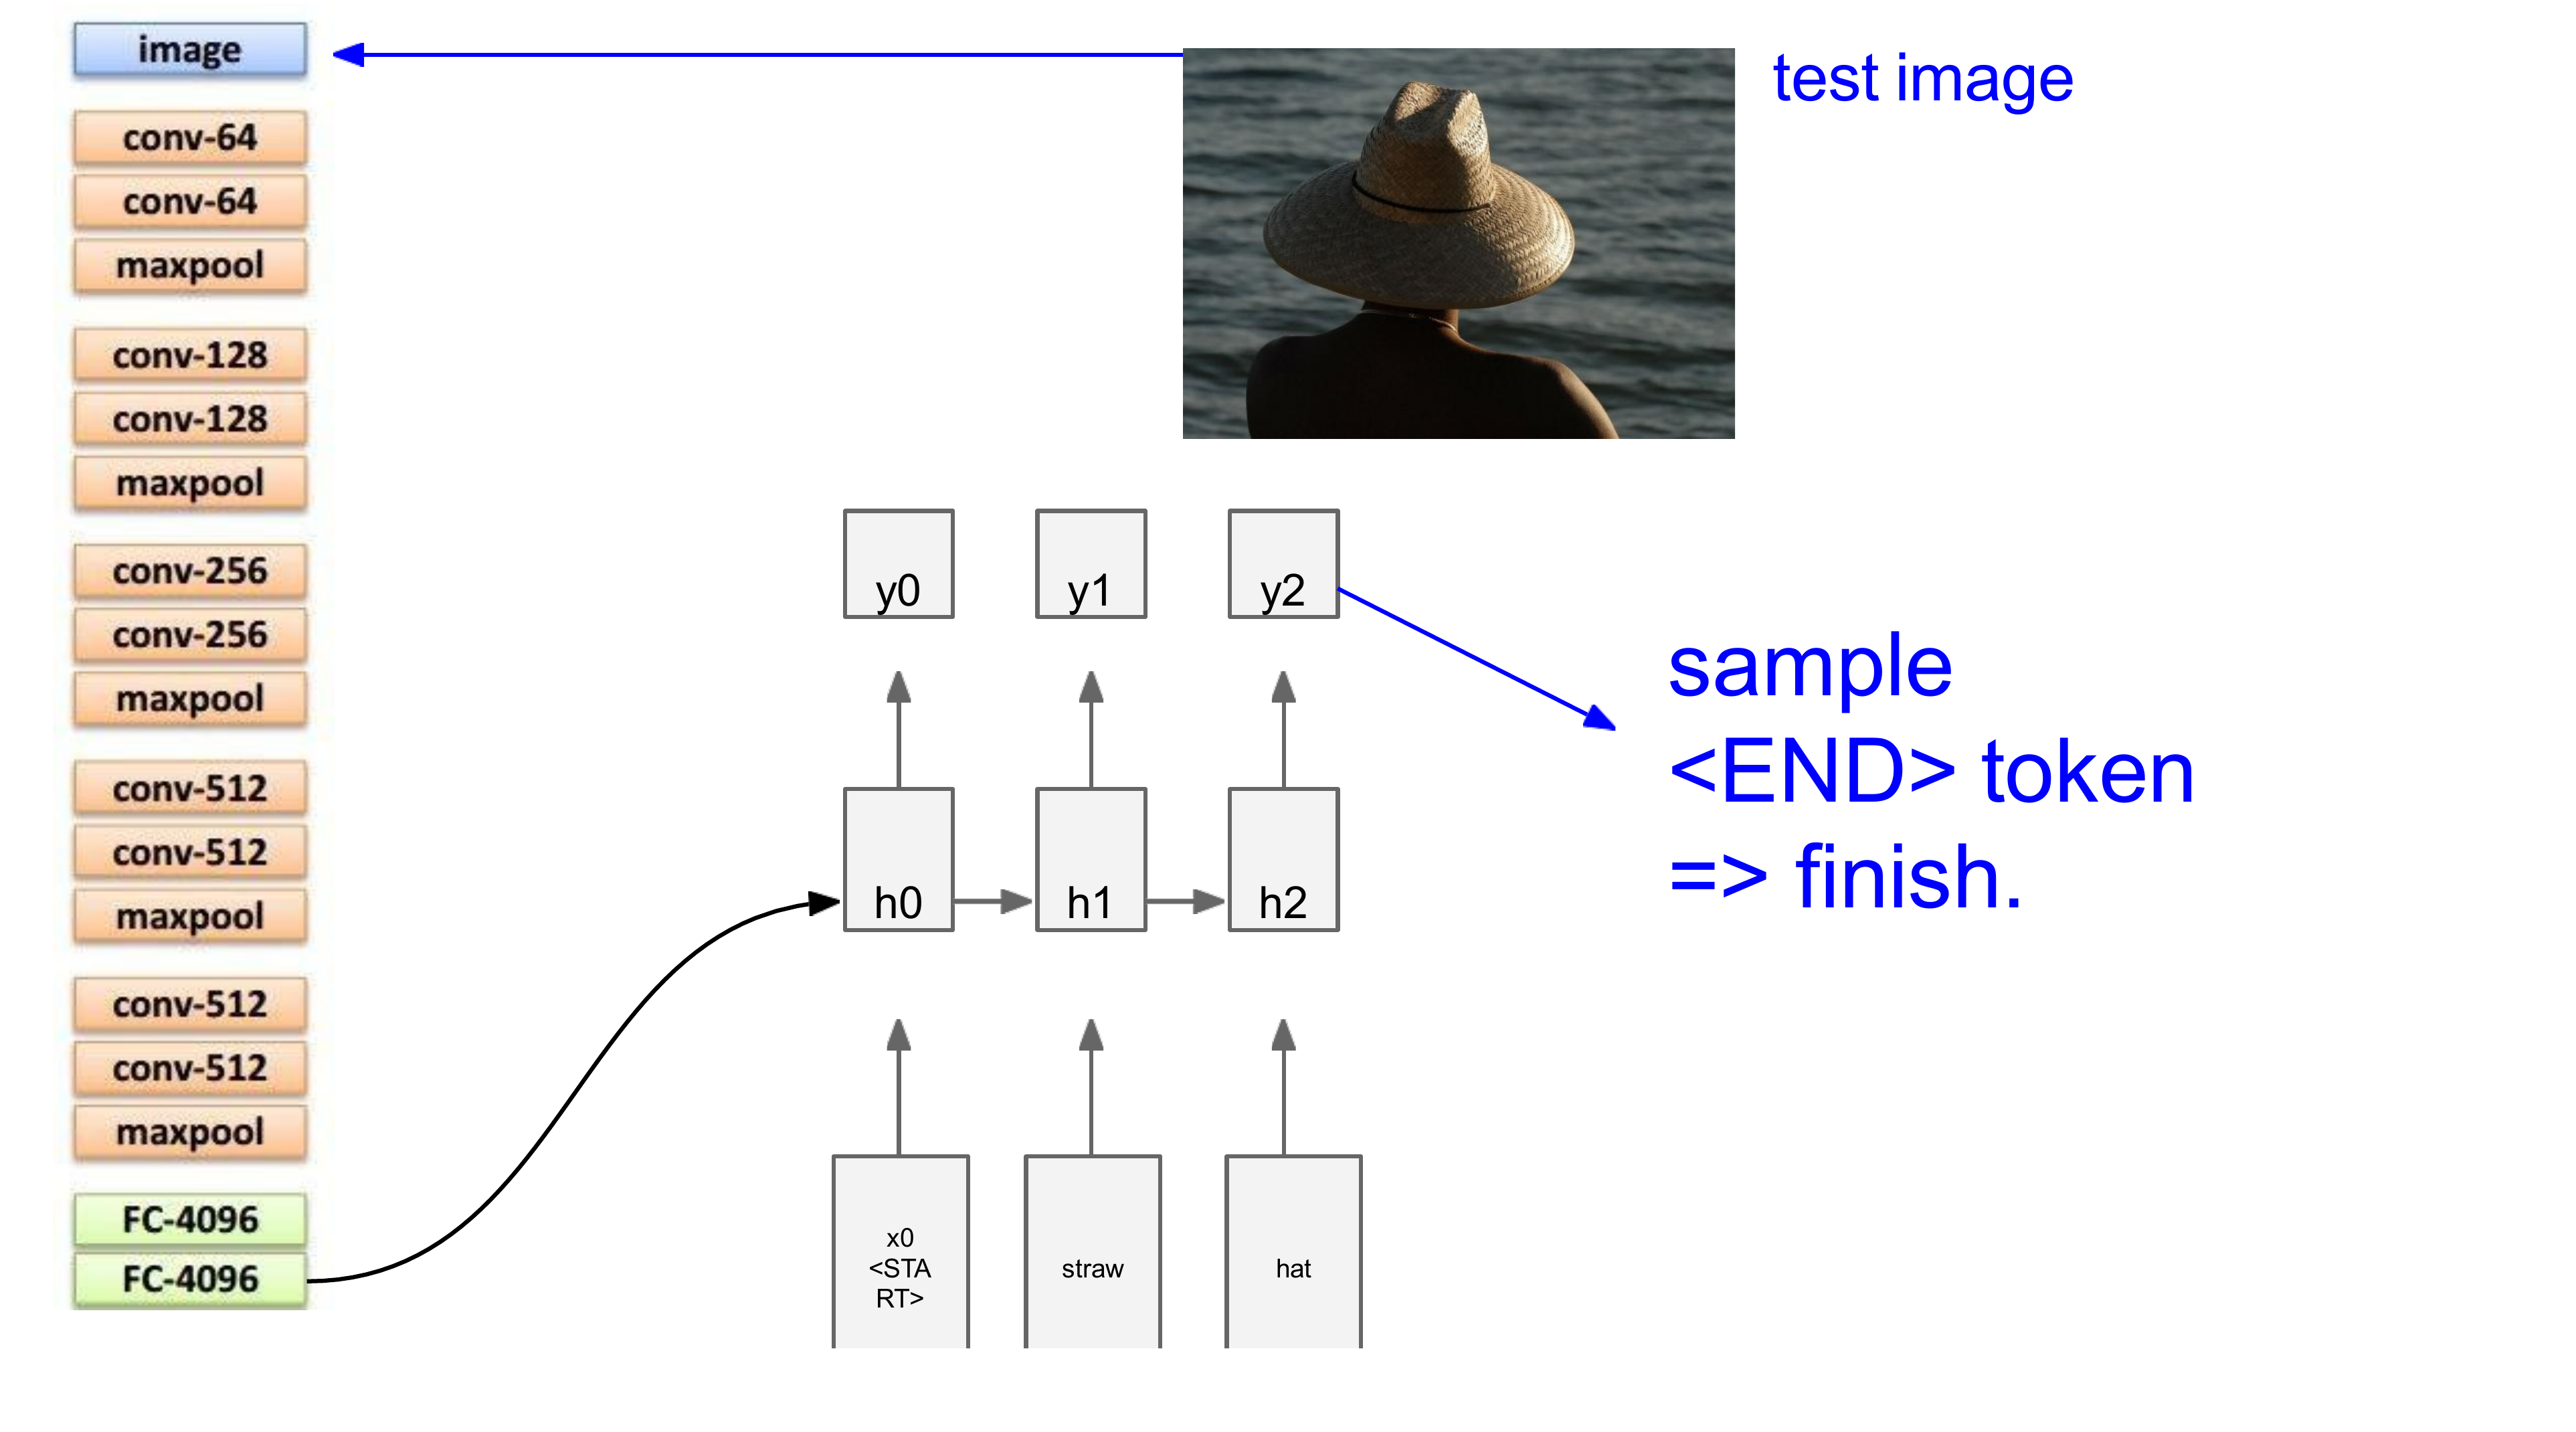
\includegraphics[width=0.72\textwidth]{Pictures/image_captioning_unrolled.png}
    \caption{Unrolled test-time generation of an image caption (Slide 123). The network generates words sequentially from a starting token until emitting the special \texttt{<END>} token.}\label{fig:captioning_unrolled}
\end{figure}

At each step, the hidden state $h_t$ projects raw scores (logits) $y_t$, which are converted into a probability distribution over the word dictionary via Softmax. Generation unfolds sequentially:
\begin{enumerate}[leftmargin=*]
    \item \textbf{Initialization ($t=0$):} Given visual vector $v$, initial memory $h_{-1} = \vec{0}$, and start token $x_0 = \texttt{<START>}$, the network computes $h_0$ and predicts distribution $y_0$. The most probable word, \textit{``straw''}, is sampled.
    \item \textbf{Sequential Steps ($t=1, 2, \dots$):} The newly sampled word is fed back as the input for the next time step alongside memory $h_t$ and visual vector $v$:
    \begin{itemize}[nosep]
        \item Feed $x_1 = \text{\textit{``straw''}} \longrightarrow$ computes $h_1 \longrightarrow$ samples \textit{``hat''}.
        \item Feed $x_2 = \text{\textit{``hat''}} \longrightarrow$ computes $h_2 \longrightarrow$ samples \texttt{<END>}.
    \end{itemize}
    \item \textbf{Stopping Criterion:} Sampling the special token \texttt{<END>} signals that the sentence is complete, terminating the autoregressive loop with final caption \textit{``straw hat''}.
\end{enumerate}

\section{Backpropagation Through Time and Gradient Flow}

Training an RNN requires computing the gradient of the total loss $L$ with respect to the shared weight matrices $W$. This process is known as \textbf{Backpropagation Through Time (BPTT)}~\cite{werbos1990backpropagation} (Slides 141--144).

\subsection{BPTT and Gradient Flow in Vanilla RNNs}

BPTT proceeds in two phases:
\begin{enumerate}
    \item \textbf{Forward Pass:} The input sequence is processed step by step, computing intermediate hidden states $h_t$ and loss terms $L_t$.
    \item \textbf{Backward Pass:} Gradients are backpropagated backward in time from step $t=T$ to $t=1$, accumulating gradient contributions to the shared weights at every step.
\end{enumerate}

When backpropagating from hidden state $h_t$ to previous state $h_{t-1}$, the gradient is multiplied by the recurrent weight matrix $W_{hh}^T$ at each step (Slides 145--147).

\subsection{Exploding and Vanishing Gradients}

Backpropagating gradients across multiple time steps involves repeated multiplication by $W_{hh}$ (neglecting the non-linearity for simplicity). As illustrated in Figure~\ref{fig:rnn_gradients}, this repeated multiplication leads to two failure modes (Slide 157):

\begin{figure}[htbp]
    \centering
    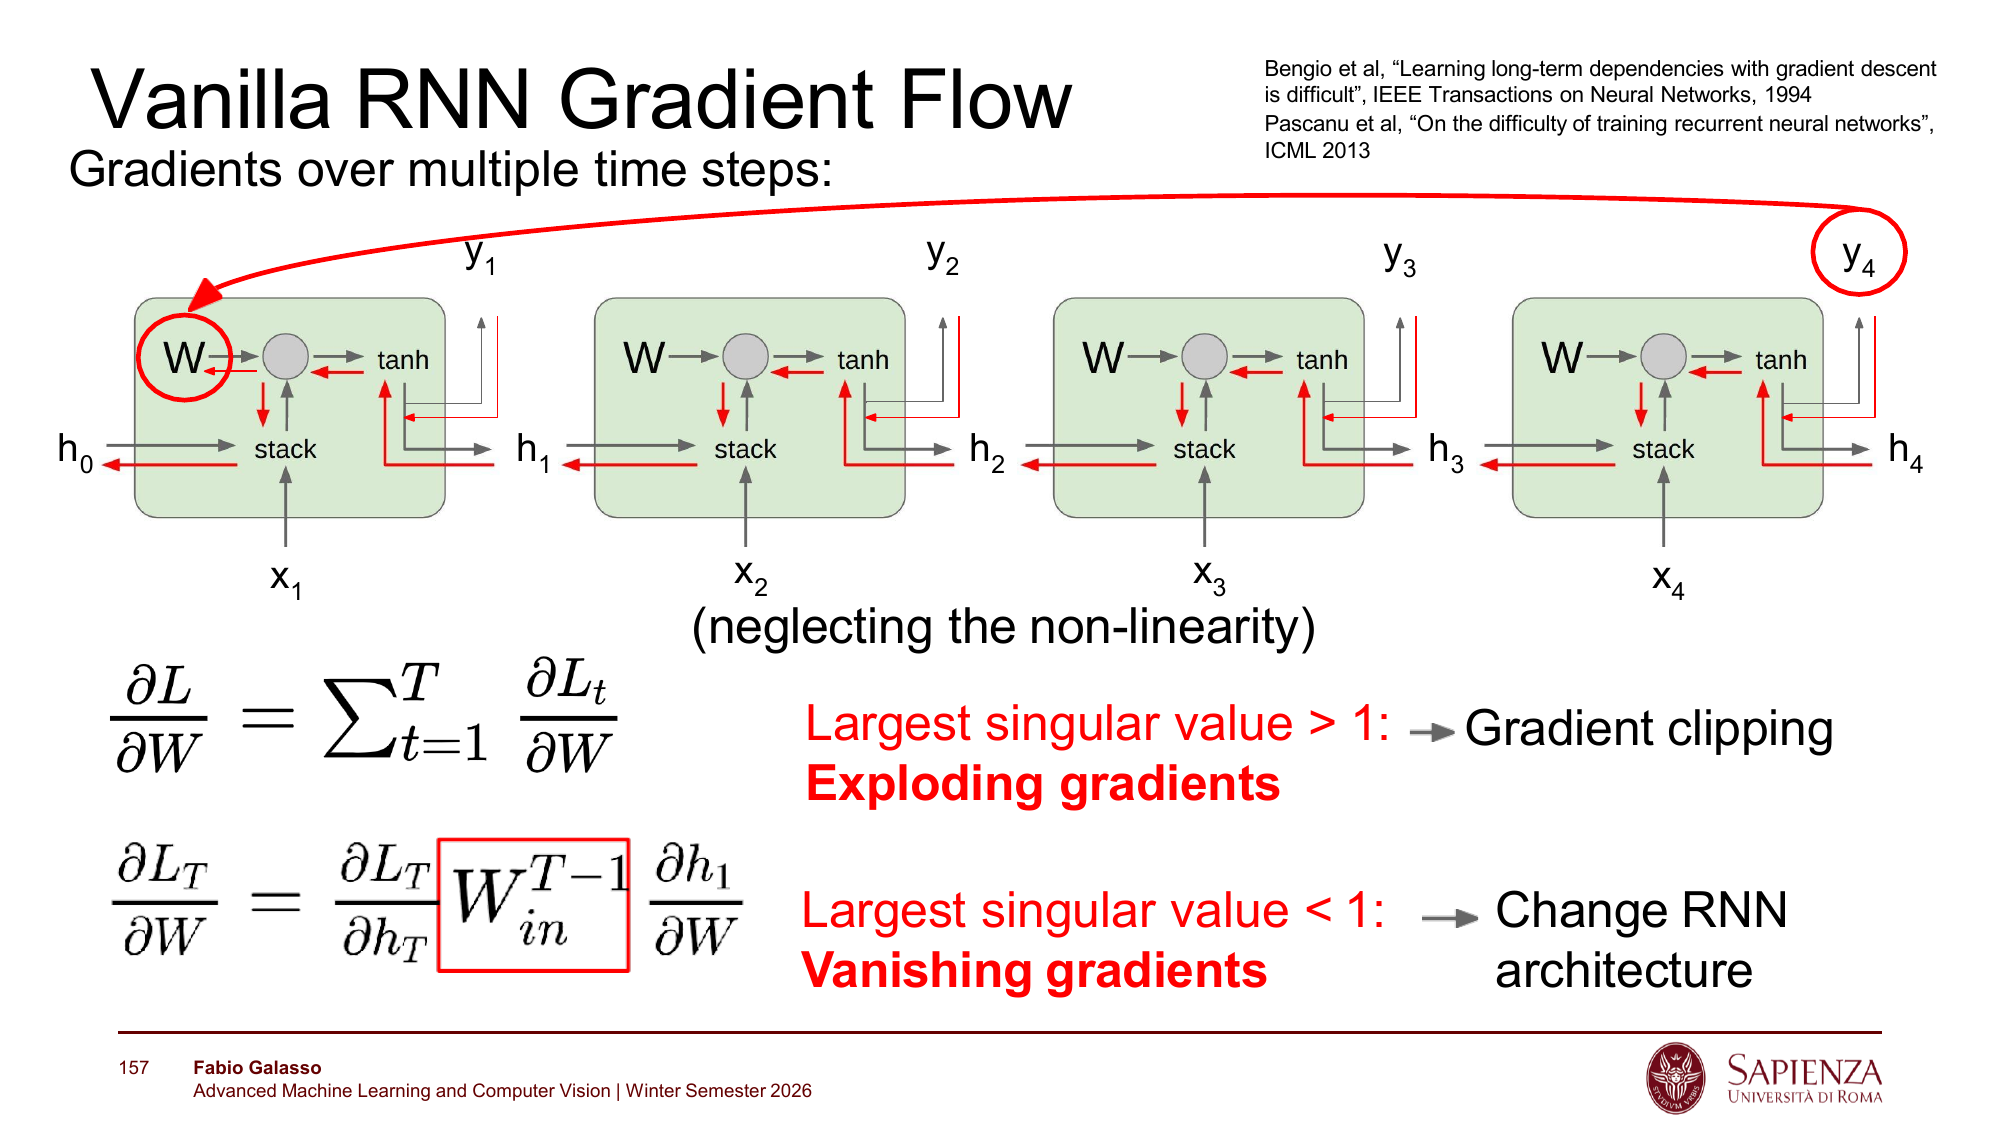
\includegraphics[width=0.82\textwidth]{Pictures/rnn_gradients.png}
    \caption{Gradient flow across multiple time steps in a Vanilla RNN (Slide 157). Repeated multiplication by $W_{hh}$ inevitably causes either exploding or vanishing gradients.}\label{fig:rnn_gradients}
\end{figure}

\begin{itemize}[leftmargin=*]
    \item \textbf{Exploding Gradients (Largest singular value $> 1$):}
    Gradients grow exponentially with sequence length, causing numerical instability.
    
    \textbf{Solution:} \textit{Gradient Clipping} (Pascanu et al., 2013)~\cite{pascanu2013difficulty}. When the gradient norm $\|g\|$ exceeds a threshold $\tau$, it is clipped:
    \[ g \longleftarrow \frac{\tau}{\|g\|} g \quad \text{if } \|g\| > \tau \]
    
    \item \textbf{Vanishing Gradients (Largest singular value $< 1$):}
    Gradients decay exponentially toward zero as they travel back in time. Early weights receive negligible updates, making it practically impossible to learn long-term dependencies.
    
    \textbf{Solution:} Vanishing gradients cannot be fixed by gradient clipping; they require redesigning the architecture with additive interactions $\longrightarrow$ \textbf{LSTM}.
\end{itemize}

\subsection{Vanilla RNN Trade-offs}

The strengths and limitations of Vanilla RNNs can be summarized as follows (Slide 158):

\begin{InsightBox}
\textbf{Vanilla RNN Trade-offs (Slide 158):}
\begin{itemize}[leftmargin=*]
    \item \textbf{Advantages:}
    \begin{itemize}[nosep]
        \item Can process input sequences of arbitrary length.
        \item Model parameter size remains strictly constant regardless of input length.
        \item Same weights are applied at every time step, providing temporal symmetry.
        \item In theory, computation at step $t$ can use information from many steps back.
    \end{itemize}
    \item \textbf{Disadvantages:}
    \begin{itemize}[nosep]
        \item Recurrent computation is slow and cannot be parallelized across time.
        \item In practice, vanishing gradients make it difficult to access information from many steps back.
    \end{itemize}
\end{itemize}
\end{InsightBox}

\section{Long Short-Term Memory}

To resolve the fatal vanishing gradient problem inherent in Vanilla RNNs, Hochreiter and Schmidhuber~\cite{hochreiter1997long} introduced the \textbf{Long Short-Term Memory (LSTM)} network.

\subsection{The Dual-State Architecture}

While a Vanilla RNN maintains only a single hidden state $h_t$, an LSTM explicitly decouples memory into two complementary internal state vectors:

\begin{enumerate}
    \item \textbf{Hidden State ($h_t$):} The short-term working state, used to emit immediate predictions and interface with adjacent layers.
    \item \textbf{Cell State ($c_t$):} The long-term persistent memory. It functions as an uninterrupted information highway where memories can flow through time with minimal linear attenuation.
\end{enumerate}

\subsection{The LSTM Cell Architecture}

Figure~\ref{fig:lstm_cell} illustrates the internal structure of the LSTM cell and its governing equations.

\begin{figure}[htbp]
    \centering
    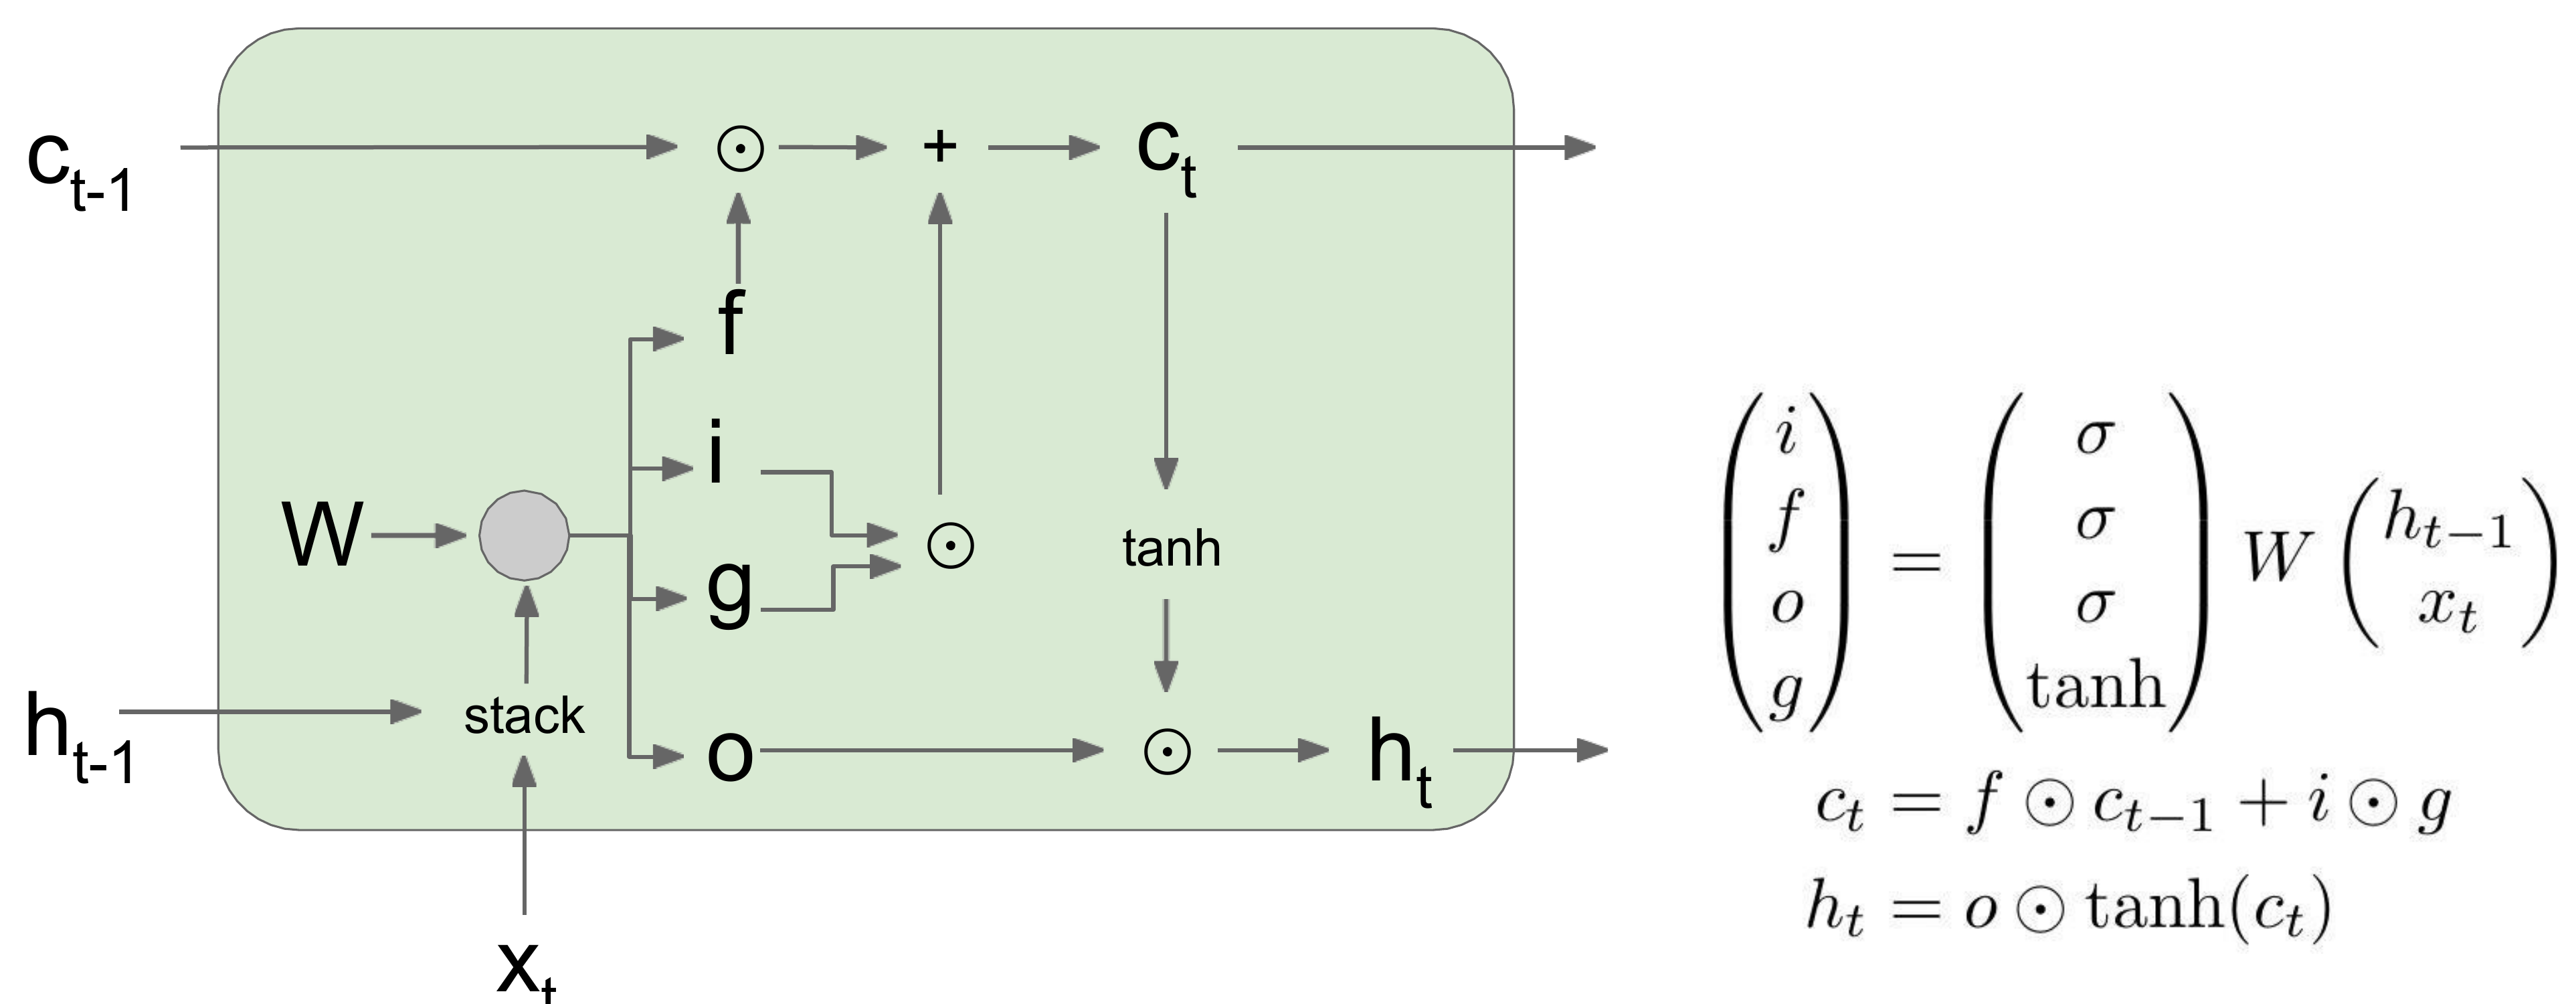
\includegraphics[width=0.98\textwidth]{Pictures/lstm_cell.png}
    \caption{The LSTM cell diagram and its update equations (from course slides). At time step $t$, the cell stacks $h_{t-1}$ and $x_t$ to compute four gates ($f, i, g, o$), updating the cell state $c_t$ additively and producing the hidden state $h_t$.}\label{fig:lstm_cell}
\end{figure}

\subsection{Detailed Breakdown of Cell Components}

To understand how information flows through the cell in Figure~\ref{fig:lstm_cell}, we can trace each input, parameter, gate, and intermediate operation:

\begin{itemize}[leftmargin=*]
    \item \textbf{Inputs to the Cell:}
    \begin{itemize}[leftmargin=1.5em]
        \item $x_t$: The input vector at the current time step $t$ (e.g., word embedding or extracted visual feature vector).
        \item $h_{t-1}$: The hidden state from the previous time step $t-1$, providing short-term context.
        \item $c_{t-1}$: The cell state from the previous time step $t-1$, carrying long-term memory along the upper horizontal highway.
    \end{itemize}

    \item \textbf{Vector Stacking and Weight Matrix $W$:}
    \begin{itemize}[leftmargin=1.5em]
        \item $\begin{pmatrix} h_{t-1} \\ x_t \end{pmatrix}$ (\textbf{stack}): Concatenates $h_{t-1}$ and $x_t$ into a single composite vector.
        \item $W$: The learnable weight matrix of the cell. Multiplying $W$ by the stacked input computes all four gate activations simultaneously in a single linear transformation:
        \[
        \begin{pmatrix} f \\ i \\ o \\ g \end{pmatrix} = \begin{pmatrix} \sigma \\ \sigma \\ \sigma \\ \tanh \end{pmatrix} W \begin{pmatrix} h_{t-1} \\ x_t \end{pmatrix}
        \]
    \end{itemize}

    \item \textbf{The Four Gating Mechanisms ($f, i, g, o$):}
    \begin{itemize}[leftmargin=1.5em]
        \item $f$ (\textbf{Forget Gate}, $\sigma$): \textit{Whether to erase cell memory}. Uses the Sigmoid activation $\sigma(z) \in [0, 1]$. Acting as a soft valve, an activation close to $0$ clears that memory dimension, whereas $1$ preserves it completely.
        \item $i$ (\textbf{Input Gate}, $\sigma$): \textit{Whether to write to the cell}. Uses Sigmoid $\sigma(z) \in [0, 1]$. It acts as a filter deciding which portions of the incoming information are relevant enough to be stored.
        \item $g$ (\textbf{Gate Gate / Candidate State}, $\tanh$): \textit{What candidate information to write}. Uses $\tanh(z) \in (-1, 1)$ to propose new candidate values to be written into the cell state.
        \item $o$ (\textbf{Output Gate}, $\sigma$): \textit{How much of the cell to reveal}. Uses Sigmoid $\sigma(z) \in [0, 1]$ to control how much of the internal cell state is exposed to the outside as the working hidden state $h_t$.
    \end{itemize}

    \item \textbf{Element-Wise Operations and State Updates:}
    \begin{itemize}[leftmargin=1.5em]
        \item $\odot$ (\textbf{Hadamard Product}): Pointwise vector multiplication used for gating. Multiplying by a $[0, 1]$ gate value smoothly scales each dimension.
        \item $f \odot c_{t-1}$: Forget gate modulation. It selectively suppresses outdated memories from the previous cell state.
        \item $i \odot g$: Input gate modulation. It scales the candidate information $g$ by the input gate $i$, letting only selected features enter the memory.
        \item $+$ (\textbf{Additive Interaction}): Merges the preserved past memory with the new candidate memory:
        \[
        c_t = f \odot c_{t-1} + i \odot g
        \]
        This addition is the core innovation of the LSTM\@: it bypasses the repeated multiplicative weight transformations of vanilla RNNs.
        \item $\tanh(c_t)$: Squashes the accumulated cell state values into $(-1, 1)$ before filtering for output.
        \item $h_t = o \odot \tanh(c_t)$: Produces the current hidden state $h_t$, which is both routed to the next time step $t+1$ and emitted upwards to produce predictions or feed higher layers.
    \end{itemize}
\end{itemize}

\subsection{Why LSTM Solves the Vanishing Gradient Problem}

The fundamental reason LSTMs succeed where Vanilla RNNs fail lies in the gradient flow along the cell state highway, illustrated in Figure~\ref{fig:lstm_gradient_flow}.

\begin{figure}[htbp]
    \centering
    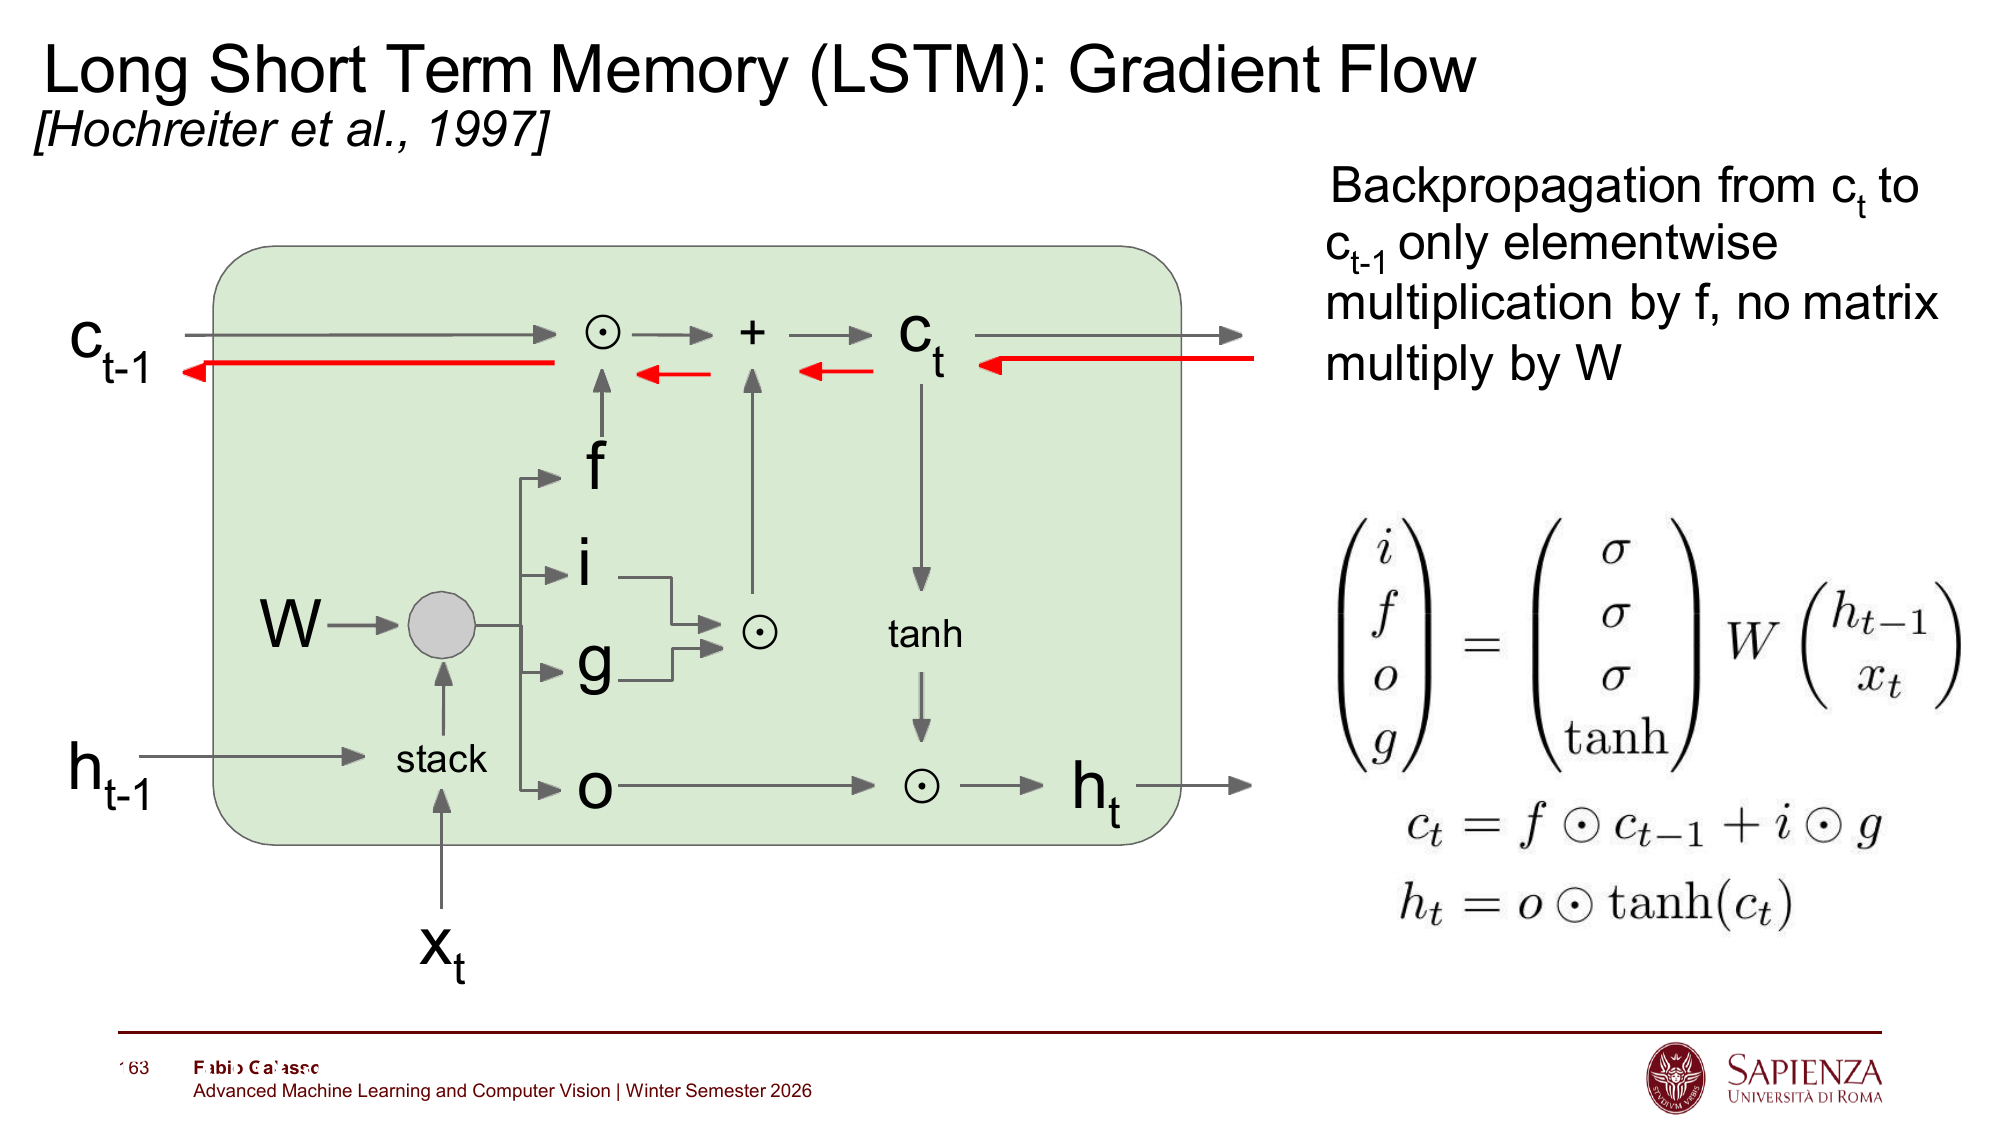
\includegraphics[width=0.72\textwidth]{Pictures/lstm_gradient_flow.png}
    \caption{Uninterrupted gradient flow along the cell state highway in an LSTM (from course slides). Backpropagation from $c_t$ to $c_{t-1}$ involves only element-wise multiplication by $f$, avoiding matrix multiplications by $W$.}\label{fig:lstm_gradient_flow}
\end{figure}

\begin{InsightBox}
\textbf{The Uninterrupted Gradient Highway: Why LSTM Overcomes Vanishing Gradients} \\
In a Vanilla RNN, backpropagating through time repeatedly multiplies error gradients by the recurrent weight matrix $W_{hh}^T$ and saturating $\tanh$ derivatives, causing the signal to decay exponentially towards zero ($W_{hh}^T \cdot W_{hh}^T \dots \to 0$).

In an LSTM, backpropagating from $c_t$ to $c_{t-1}$ along the upper cell state highway yields $\frac{\partial c_t}{\partial c_{t-1}} = f$:
\begin{itemize}[leftmargin=*]
    \item \textbf{No Weight Matrix Multiplications:} Backpropagation along the highway involves only an element-wise multiplication by the forget gate vector $f$, with \textbf{no matrix multiplication by $W$}. There is no risk of exponential degradation caused by repeated matrix powers.
    \item \textbf{Selective Memory Retention ($f \approx 1$):} The forget gate outputs values in $[0, 1]$. If the network learns that an early piece of context is critical and sets $f \approx 1$, the local gradient derivative is practically $1$.
    \item \textbf{Lossless Flow Across Hundreds of Steps:} Multiplying by $1$ repeatedly preserves the error magnitude:
    \[ 1 \times 1 \times \cdots \times 1 = 1 \]
    The gradient signal flows backwards through dozens or hundreds of time steps virtually intact!
    \item \textbf{The ResNet Analogy:} Just as ResNets use additive identity skip connections ($x + F(x)$) to bypass deep spatial layers, LSTMs use an additive cell state ($f \odot c_{t-1} + i \odot g$) to bypass long temporal sequences.
\end{itemize}
\end{InsightBox}

\newpage
\section{Chapter Summary and Conceptual Graph}

The concepts developed in this chapter trace the evolution of sequence models from parallel temporal convolutions to recurrent memory networks and additive gradient highways:

\begin{InsightBox}
\textbf{The Logical Connections Between Nodes:}
\begin{itemize}[leftmargin=*]
    \item \textbf{From Node 1 to 2:} Handling variable-length sequences with temporal ordering prompts using 1D convolutions; enforcing causality prevents future lookahead, while dilation expands context without sacrificing parallel training.
    \item \textbf{From Node 2 to 3:} Despite their parallel speed, TCNs have a fixed receptive field buffer; Recurrent Neural Networks introduce true dynamic memory via an evolving hidden state $h_t$ with parameter sharing.
    \item \textbf{From Node 3 to 4:} Training recurrent graphs requires unrolling them through time and calculating loss gradients backwards across all time steps via Backpropagation Through Time (BPTT).
    \item \textbf{From Node 4 to 5:} Unrolling across long horizons exposes BPTT to repeated multiplications by $W_{hh}^{T-1}$. If the spectral radius exceeds 1, gradients explode (controlled via Gradient Clipping); if less than 1, gradients vanish exponentially.
    \item \textbf{From Node 5 to 6:} Because vanishing gradients represent an architectural failure of Vanilla RNNs, Hochreiter and Schmidhuber redesigned the memory cell: separating working state $h_t$ from a dedicated cell state $c_t$.
    \item \textbf{From Node 6 to 7:} Regulating the cell state via input, forget, and output gates ($i, f, o$) and applying purely additive updates ($+$) establishes an uninterrupted gradient highway, allowing LSTMs to preserve long-range dependencies across hundreds of steps.
\end{itemize}
\end{InsightBox}

\begin{figure}[htbp]
\centering
\begin{tikzpicture}[
    node distance=0.6cm and 0cm,
    conceptnode/.style={
        rectangle, rounded corners=4pt, draw=ocre!80, fill=ocre!8,
        line width=0.8pt, text width=0.85\textwidth, inner sep=5pt,
        font=\sffamily\small
    },
    arrowline/.style={
        ->, >=Stealth, line width=1pt, color=ocre!80
    }
]

\node[conceptnode] (n1) {\textbf{1. Sequential \& Temporal Data}\\
Variable-length ordered tokens/timesteps requiring dynamic input/output mappings (Seq2Seq, forecasting).};

\node[conceptnode, below=of n1] (n2) {\textbf{2. Temporal Convolutional Networks (TCN)}\\
Applies parallel 1D convolutions; enforces strict causality and exponential dilation to expand receptive fields.};

\node[conceptnode, below=of n2] (n3) {\textbf{3. Recurrent Neural Networks (RNN)}\\
Maintains an internal hidden state ($h_t$) as dynamic memory, reusing transition parameters $W$ across all steps.};

\node[conceptnode, below=of n3] (n4) {\textbf{4. Backpropagation Through Time (BPTT)}\\
Unrolls computation across time, backpropagating gradients through repeated multiplications of $W_{hh}$.};

\node[conceptnode, below=of n4] (n5) {\textbf{5. Gradient Failure: Vanishing \& Exploding}\\
Powers $W_{hh}^{T-1}$ cause exploding gradients (fixed by clipping) or vanishing gradients (structural amnesia).};

\node[conceptnode, below=of n5] (n6) {\textbf{6. LSTM Dual-State Architecture}\\
Explicitly decouples short-term working output ($h_t$) from an uninterrupted long-term cell state ($c_t$).};

\node[conceptnode, below=of n6] (n7) {\textbf{7. Gating Valves \& Additive Highway}\\
Sigmoid gates ($i, f, o$) modulate information flow; additive cell updates eliminate matrix multiplications and prevent gradient decay.};

\draw[arrowline] (n1) -- (n2);
\draw[arrowline] (n2) -- (n3);
\draw[arrowline] (n3) -- (n4);
\draw[arrowline] (n4) -- (n5);
\draw[arrowline] (n5) -- (n6);
\draw[arrowline] (n6) -- (n7);

\end{tikzpicture}
\caption{Conceptual roadmap of sequence modeling, recurrent dynamics, and LSTMs.}\label{fig:ch3_roadmap}
\end{figure}
